% ******************************* PhD Thesis Template **************************
% Please have a look at the README.md file for info on how to use the template

\documentclass[letterpaper,12pt,times,oneside,numbered,print,index,custommargin,PageStyleI]{Classes/PhDThesisPSnPDF}

% ******************************************************************************
% ******************************* Class Options ********************************
% *********************** See README for more details **************************
% ******************************************************************************

% `a4paper'(The University of Cambridge PhD thesis guidelines recommends a page
% size a4 - default option) or `a5paper': A5 Paper size is also allowed as per
% the Cambridge University Engineering Deparment guidelines for PhD thesis
%
% `11pt' or `12pt'(default): Font Size 10pt is NOT recommended by the University
% guidelines
%
% `oneside' or `twoside'(default): Printing double side (twoside) or single
% side.
%
% `print': Use `print' for print version with appropriate margins and page
% layout. Leaving the options field blank will activate Online version.
%
% `index': For index at the end of the thesis
%
% `draftclassic': For draft mode without loading any images (same as draft in book)
%
% `draft': Special draft mode with line numbers, images, and water mark with
% timestamp and custom text. Position of the text can also be modified.
%
% `abstract': To generate only the title page and abstract page with
% dissertation title and name, to submit to the Student Registry
%
% `chapter`: This option enables only the specified chapter and it's references
%  Useful for review and corrections.
%
% ************************* Custom Page Margins ********************************
%
% `custommargin`: Use `custommargin' in options to activate custom page margins,
% which can be defined in the preamble.tex. Custom margin will override
% print/online margin setup.
%
% *********************** Choosing the Fonts in Class Options ******************
%
% `times' : Times font with math support. (The Cambridge University guidelines
% recommend using times)
%
% `fourier': Utopia Font with Fourier Math font (Font has to be installed)
%            It's a free font.
%
% `customfont': Use `customfont' option in the document class and load the
% package in the preamble.tex
%
% default or leave empty: `Latin Modern' font will be loaded.
%
% ********************** Choosing the Bibliography style ***********************
%
% `authoryear': For author-year citation eg., Krishna (2013)
%
% `numbered': (Default Option) For numbered and sorted citation e.g., [1,5,2]
%
% `custombib': Define your own bibliography style in the `preamble.tex' file.
%              `\RequirePackage[square, sort, numbers, authoryear]{natbib}'.
%              This can be also used to load biblatex instead of natbib
%              (See Preamble)
%
% **************************** Choosing the Page Style *************************
%
% `default (leave empty)': For Page Numbers in Header (Left Even, Right Odd) and
% Chapter Name in Header (Right Even) and Section Name (Left Odd). Blank Footer.
%
% `PageStyleI': Chapter Name next & Page Number on Even Side (Left Even).
% Section Name & Page Number in Header on Odd Side (Right Odd). Footer is empty.
%
% `PageStyleII': Chapter Name on Even Side (Left Even) in Header. Section Number
% and Section Name in Header on Odd Side (Right Odd). Page numbering in footer

% Uncomment to change page style
%\pagestyle{PageStyleII}

\usepackage[spanish,english]{babel}
% ********************************** Preamble **********************************
% Preamble: Contains packages and user-defined commands and settings
% ******************************************************************************
% ****************************** Custom Margin *********************************

% Add `custommargin' in the document class options to use this section
% Set {innerside margin / outerside margin / topmargin / bottom margin}  and
% other page dimensions
\ifsetCustomMargin
  \RequirePackage[left=37mm,right=30mm,top=35mm,bottom=30mm]{geometry}
  \setFancyHdr % To apply fancy header after geometry package is loaded
\fi

% Add spaces between paragraphs
%\setlength{\parskip}{0.5em}
% Ragged bottom avoids extra whitespaces between paragraphs
\raggedbottom
% To remove the excess top spacing for enumeration, list and description
%\usepackage{enumitem}
%\setlist[enumerate,itemize,description]{topsep=0em}

% *****************************************************************************
% ******************* Fonts (like different typewriter fonts etc.)*************

% Add `customfont' in the document class option to use this section

\ifsetCustomFont
  % Set your custom font here and use `customfont' in options. Leave empty to
  % load computer modern font (default LaTeX font).
  %\RequirePackage{helvet}

  % For use with XeLaTeX
  %  \setmainfont[
  %    Path              = ./libertine/opentype/,
  %    Extension         = .otf,
  %    UprightFont = LinLibertine_R,
  %    BoldFont = LinLibertine_RZ, % Linux Libertine O Regular Semibold
  %    ItalicFont = LinLibertine_RI,
  %    BoldItalicFont = LinLibertine_RZI, % Linux Libertine O Regular Semibold Italic
  %  ]
  %  {libertine}
  %  % load font from system font
  %  \newfontfamily\libertinesystemfont{Linux Libertine O}
\fi

% *****************************************************************************
% **************************** Custom Packages ********************************
\usepackage{bm}
\usepackage{bbm}
\usepackage{amsfonts}
\usepackage{amsmath}
\usepackage{amssymb}
\usepackage{siunitx} % use this package module for SI units
%\RequirePackage{amstext}
%\RequirePackage{amsbsy}
%\RequirePackage{amsopn}
%\RequirePackage{gensymb}
%\RequirePackage[cmex10]{amsmath}
\RequirePackage[sumlimits,cmex10]{mathtools}
%\usepackage[sumlimits]{mathtools}
\usepackage{cancel}
%\renewcommand\CancelColor{\color{darkblue}}
%\renewcommand\CancelColor{\color{lightred}}

\newcommand{\op}{\wedge}

\newcommand{\field}[1]{\mathbb{#1}} % requires amsfonts
\newcommand{\pd}[2]{\frac{\partial#1}{\partial#2}}

\newcommand{\vecbi}[1]{\boldsymbol{#1}}
\renewcommand{\vec}[1]{\bm{#1}}
\newcommand{\pp}{\mathbbm{P}}
\newcommand{\rr}{\mathbbm{R}}
\newcommand{\sss}{\mathbbm{S}}
\newcommand{\Aa}{\mathbb{a}}
\newcommand{\bb}{\mathbb{b}}
\newcommand{\cc}{\mathbb{c}}
\newcommand{\dd}{\mathbb{d}}
\newcommand{\xx}{\mathbbm{x}}
\newcommand{\sv}{\mathbbm{s}}
\newcommand{\av}{\mathbbm{a}}
\newcommand{\bv}{\mathbbm{b}}
\newcommand{\cv}{\mathbbm{c}}
\newcommand{\dv}{\mathbbm{d}}
\newcommand{\uv}{\mathbbm{u}}
\newcommand{\yy}{\mathbb{y}}
\newcommand{\vv}{\mathbb{v}}
\newcommand{\pl}{\mathbb{p}}
\newcommand{\nn}{\mathbb{n}}
\newcommand{\pipi}{\mathbbm{\Pi}}
\newcommand{\ts}{\mathbbm{T}}
%\DeclareMathSizes{10}{10}{7}{5}
%\DeclareMathSizes{11}{11}{7.7}{5.5}
%\DeclareMathSizes{12}{12}{8.4}{6}
%\DeclareMathSizes{13}{13}{9.1}{6.5}
%\DeclareMathSizes{14}{14}{9.8}{7}

% ************************* Algorithms and Pseudocode **************************

%\usepackage{algpseudocode}


% ********************Captions and Hyperreferencing / URL **********************

% Captions: This makes captions of figures use a boldfaced small font.
%\RequirePackage[small,bf]{caption}

\RequirePackage[labelsep=space,tableposition=top]{caption}
\renewcommand{\figurename}{Fig.} %to support older versions of captions.sty


% *************************** Graphics and figures *****************************

%\usepackage{rotating}
%\usepackage{wrapfig}

% Uncomment the following two lines to force Latex to place the figure.
% Use [H] when including graphics. Note 'H' instead of 'h'
%\usepackage{float}
%\restylefloat{figure}

% Subcaption package is also available in the sty folder you can use that by
% uncommenting the following line
% This is for people stuck with older versions of texlive
%\usepackage{sty/caption/subcaption}
\usepackage{subcaption}

% ********************************** Tables ************************************
\usepackage{booktabs} % For professional looking tables
\usepackage{multirow}

%\usepackage{multicol}
%\usepackage{longtable}
%\usepackage{tabularx}


% *********************************** SI Units *********************************
\usepackage{siunitx} % use this package module for SI units


% ******************************* Line Spacing *********************************

% Choose linespacing as appropriate. Default is one-half line spacing as per the
% University guidelines

% \doublespacing
% \onehalfspacing
% \singlespacing


% ************************ Formatting / Footnote *******************************

% Don't break enumeration (etc.) across pages in an ugly manner (default 10000)
%\clubpenalty=500
%\widowpenalty=500

%\usepackage[perpage]{footmisc} %Range of footnote options


% *****************************************************************************
% *************************** Bibliography  and References ********************

%\usepackage{cleveref} %Referencing without need to explicitly state fig /table

% Add `custombib' in the document class option to use this section
\ifuseCustomBib
   \RequirePackage[square, sort, numbers, authoryear]{natbib} % CustomBib

% If you would like to use biblatex for your reference management, as opposed to the default `natbibpackage` pass the option `custombib` in the document class. Comment out the previous line to make sure you don't load the natbib package. Uncomment the following lines and specify the location of references.bib file

%\RequirePackage[backend=biber, style=numeric-comp, citestyle=numeric, sorting=nty, natbib=true]{biblatex}
%\bibliography{References/references} %Location of references.bib only for biblatex

\fi

% changes the default name `Bibliography` -> `References'
%\renewcommand{\bibname}{References}


% ******************************************************************************
% ************************* User Defined Commands ******************************
% ******************************************************************************

%% *********** To change the name of Table of Contents / LOF and LOT ************
%
%\renewcommand{\chaptername}{Capítulo}
%\renewcommand{\contentsname}{Table de Contenidos}
%\renewcommand{\listfigurename}{Lista de Figuras}
%\renewcommand{\listtablename}{Lista de Tablas}
%% changes the default name `Bibliography` -> `References'
%\renewcommand{\bibname}{Bibliografía}

% ********************** TOC depth and numbering depth *************************

\setcounter{secnumdepth}{3}
\setcounter{tocdepth}{3}


% ******************************* Nomenclature *********************************

% To change the name of the Nomenclature section, uncomment the following line

%\renewcommand{\nomname}{Symbols}


% ********************************* Appendix ***********************************

% The default value of both \appendixtocname and \appendixpagename is `Appendices'. These names can all be changed via:

%\renewcommand{\appendixtocname}{List of appendices}
%\renewcommand{\appendixname}{Appndx}

% *********************** Configure Draft Mode **********************************

% Uncomment to disable figures in `draft'
%\setkeys{Gin}{draft=true}  % set draft to false to enable figures in `draft'

% These options are active only during the draft mode
% Default text is "Draft"
%\SetDraftText{DRAFT}

% Default Watermark location is top. Location (top/bottom)
%\SetDraftWMPosition{bottom}

% Draft Version - default is v1.0
%\SetDraftVersion{v1.1}

% Draft Text grayscale value (should be between 0-black and 1-white)
% Default value is 0.75
%\SetDraftGrayScale{0.8}


% ******************************** Todo Notes **********************************
%% Uncomment the following lines to have todonotes.

%\ifsetDraft
%	\usepackage[colorinlistoftodos]{todonotes}
%	\newcommand{\mynote}[1]{\todo[author=kks32,size=\small,inline,color=green!40]{#1}}
%\else
%	\newcommand{\mynote}[1]{}
%	\newcommand{\listoftodos}{}
%\fi

% Example todo: \mynote{Hey! I have a note}


% ************************ Thesis Information & Meta-data **********************
% Thesis title and author information, refernce file for biblatex
% ************************ Thesis Information & Meta-data **********************
%% The title of the thesis
\title{Implementación de un motor de juego en lenguajes puramente funcionales}
%\texorpdfstring is used for PDF metadata. Usage:
%\texorpdfstring{LaTeX_Version}{PDF Version (non-latex)} eg.,
%\texorpdfstring{$sigma$}{sigma}

%% Subtitle (Optional)
%\subtitle{Using the CUED template}

%% The full name of the author
\author{José Daniel Duran Toro}

%% Department (eg. Department of Engineering, Maths, Physics)
\dept{Departamento de Computación y Tecnología de la Información}

%% University and Crest
\university{Universidad Simón Bolívar}
% Crest minimum should be 30mm.
\crest{
\includegraphics[width=0.2\textwidth]{University_Crest}}
%% Use this crest, if you are using the college crest
%% Crest long miminum should be 65mm
%\crest{
\includegraphics[width=0.45\textwidth]{University_Crest_Long}}

%% College shield [optional]
% Crest minimum should be 30mm.
%\collegeshield{
\includegraphics[width=0.2\textwidth]{CollegeShields/Kings}}


%% Supervisor (optional)
%% for multiple supervisors, append each supervisor with the \newline command
%\supervisor{Prof. A.B. Supervisor\newline
%Prof. C.D. Supervisor}

%% Supervisor Role (optional) - Supervisor (default) or advisor
% \supervisorrole{\textbf{Supervisors: }}
%% if no title is desired:
% \supervisorrole{}

%% Supervisor line width: required to align supervisors
%\supervisorlinewidth{0.35\textwidth}

%% Advisor (optional)
%% for multiple advisors, append each advisor with the \newline command
%\advisor{Dr. A. Advisor\newline
%Dr. B. Advisor}

%% Advisor Role (optional) - Advisor (default) or leave empty
% \advisorrole{Advisors: }
%% if no title is required
% \advisorrole{}

%% Advisor line width: required to align supervisors
%\advisorlinewidth{0.25\textwidth}


%% You can redefine the submission text:
% Default as per the University guidelines:
% ``This dissertation is submitted for the degree of''
\renewcommand{\submissiontext}{Trabajo Especial de Grado \\
para obtener el título de \\
~~ \\%
 }

%% Full title of the Degree
\degreetitle{Ingeniero de la Computación}

%% College affiliation (optional)
%\college{King's College}

%% Submission date
% Default is set as {\monthname[\the\month]\space\the\year}
\degreedate{Diciembre 2017}

%% Meta information
\subject{GameEngine} \keywords{{Game Engine} {Haskell} {Functional Programming} {Universidad Simón Bolívar}}


% ***************************** Abstract Separate ******************************
% To printout only the titlepage and the abstract with the PhD title and the
% author name for submission to the Student Registry, use the `abstract' option in
% the document class.

\ifdefineAbstract
 \pagestyle{empty}
 \includeonly{Declaration/declaration, Abstract/abstract}
\fi

% ***************************** Chapter Mode ***********************************
% The chapter mode allows user to only print particular chapters with references
% Title, Contents, Frontmatter are disabled by default
% Useful option to review a particular chapter or to send it to supervisior.
% To use choose `chapter' option in the document class

\ifdefineChapter
 \includeonly{Chapter3/chapter3}
\fi

% ******************************** Front Matter ********************************
\begin{document}
\selectlanguage{spanish}
\lstset{
basicstyle =\scriptsize,          % print whole listing small
keywordstyle =\color{black}\bfseries, % underlined bold black keywords  basicstyle=\ttfamily,
  columns=fullflexible,
  frame=single,
  breaklines=true,
  postbreak=\mbox{\textcolor{red}{$\hookrightarrow$}\space},
}

\frontmatter

\graphicspath{{Figs/}}
\begin{titlepage}

\begin{figure}[!htbp!]
\centering

\includegraphics[width=0.2\textwidth]{University_Crest}
\end{figure}

\begin{center}

\Large UNIVERSIDAD SIMÓN BOLÍVAR\\
\large \textbf {DECANATO DE ESTUDIOS PROFESIONALES}\\
\large \textbf {COORDINACIÓN DE INGENIERÍA DE LA COMPUTACIÓN}\\

\vfill
\large \textbf {IMPLEMENTACIÓN DE UN MOTOR DE JUEGO EN LENGUAJES PURAMENTE FUNCIONALES}

\vfill
Por:\\
José Daniel Duran Toro

\vfill
Realizado con la asesoría de:\\
Victor Theoktisto

\vfill
\large PROYECTO DE GRADO\\
Presentado ante la Ilustre Universidad Simón Bolívar\\
como requisito parcial para optar al título de\\
Ingeniero de la Computación

\vfill
\textbf {Sartenejas, Enero 2018}

\end{center}

\end{titlepage}

% *********** To change the name of Table of Contents / LOF and LOT ************

%\renewcommand{\chaptername}{Capítulo}
%\renewcommand{\contentsname}{Índice de Contenidos}
%\renewcommand{\listfigurename}{Lista de Figuras}
%\renewcommand{\listtablename}{Lista de Tablas}
%% changes the default name `Bibliography` -> `References'
%\renewcommand{\bibname}{Bibliografía}
%\renewcommand{\abstractname}{Resumen}
%\renewcommand{\abstractname}{Resumen}
%% ******************************* Thesis Dedidcation ********************************

\begin{dedication} 

I would like to dedicate this thesis to my loving parents \dots

\end{dedication}


%% ******************************* Thesis Declaration ***************************

\begin{declaration}

I hereby declare that except where specific reference is made to the work of 
others, the contents of this dissertation are original and have not been 
submitted in whole or in part for consideration for any other degree or 
qualification in this, or any other university. This dissertation is my own 
work and contains nothing which is the outcome of work done in collaboration 
with others, except as specified in the text and Acknowledgements. This 
dissertation contains fewer than 65,000 words including appendices, 
bibliography, footnotes, tables and equations and has fewer than 150 figures.

% Author and date will be inserted automatically from thesis.tex \author \degreedate

\end{declaration}


%% ************************** Thesis Acknowledgements **************************

\begin{acknowledgements}      


And I would like to acknowledge ...


\end{acknowledgements}

% ************************** Thesis Abstract *****************************
% Use `abstract' as an option in the document class to print only the titlepage and the abstract.
\begin{abstract}

La industria moderna de videojuegos maneja algunos de los proyectos más grandes y complejos llevados a cabos en el área de la informática, y con los riesgos financieros que estos proyectos implican, llevan a esta industria a la búsqueda de nuevas formas de aumentar la productividad, reducir errores y adaptar nuevas y cambiantes tecnologías a los ciclos de desarrollo de juegos. Sin embargo, en la actualidad esta industria sufre de ciclos de desarrollo cortos con equipos que comprendes miles de personas, llevando a código que muchas veces contiene fallas o es lo suficientemente complicado para hacer imposible su crecimiento y expansión.

El presente trabajo propone una alternativa para la producción de videojuegos en la forma de un motor de juego que permita la producción de los mismos en un lenguaje funcional, en este caso el lenguaje Haskell, para así poder hacer uso de las ventajas que este tipo de lenguajes, como la facilidad para crear código paralelo y la seguridad de tipos, para proveer así de una mejora en la productividad y calidad de los juegos creados.

En el lenguaje funcional Haskell se ha producido diversos juegos a pequeña escala, e inclusive se ha visto motores de juego simples, como por ejemplo Helm, Bogre-Banana y actionkid, pero ninguno de estos programas explota las capacidades del lenguaje como en el caso del paralelismo y, en el caso de los motores, de la seguridad de tipos que se puede obtener al usar funciones puras.

A lo largo de este proyecto, se creó un motor de juego funcional siguiendo una metodologia de desarrollo dirigida por prototipos. El prototipo creado en el desarrollo de este trabajo usa el paradigma de programación funcional reactiva como substituto del sistema entidad-componente popular en la industria de videojuegos. Este paradigma permite a los objetos del juego ser representados como cómputos puros en el contexto de Haskell, lo que permite al motor y al compilador realizar mejoras en la corrida del juego.

El motor también permite, en forma transparente al programador, ejecutar código en forma concurrente llevando a una mejora en el rendimiento de los juegos creados y así a la experiencia de juego. En resumidas cuentas, un motor de juego puede beneficiarse de usar un lenguaje funcional como base y permitir al programador enfocarse en la jugabilidad mientras que el motor garantiza una mayor correctitud del código y a la vez que hace un mayor uso de los recursos del sistema. Futuras mejoras de este motor pueden enfocarse en agregar funcionalidades en la forma de subsistemas, como un motor de física o de inteligencia artificial, o en mejorar la usabilidad.

\end{abstract}


% *********************** Adding TOC and List of Figures ***********************

\tableofcontents

\listoffigures

\listoftables

% \printnomenclature[space] space can be set as 2em between symbol and description
%\printnomenclature[3em]

\nomenclature{$ECS$}{Patrón Sistema Entidad Componente.}
\nomenclature{$API$}{Interfaces de programación de aplicación.}
\nomenclature{$GPU$}{Unidad de procesamiento de gráficos.}
\nomenclature{$CPU$}{Unidad de procesamiento central.}
\nomenclature{$NPC$}{Personaje no jugable -- Non player character}
\nomenclature{$FRP$}{Programación Funcional Reactiva - Functional reactive programming}

\printnomenclature

% ******************************** Main Matter *********************************
\mainmatter

\chapter{Introducción}
\label{capitulo1}

La industria moderna de videojuegos maneja algunos de los proyectos más grandes y complejos llevados a cabos en el área de la informática, y con los riesgos financieros que estos proyectos implican, llevan a esta industria a la búsqueda de nuevas formas de aumentar la productividad, reducir errores y adaptar nuevas y cambiantes tecnologías a los ciclos de desarrollo de juegos. Sin embargo, en la actualidad esta industria sufre de ciclos de desarrollo cortos con equipos que comprendes miles de personas, llevando a código que muchas veces contiene fallas o es lo suficientemente complicado para hacer imposible su crecimiento y expansión.

El presente trabajo propone una alternativa para la producción de videojuegos en la forma de un motor de juego que permita la producción de los mismos en un lenguaje funcional, en este caso el lenguaje \emph{Haskell}, para así poder hacer uso de las ventajas que este tipo de lenguajes, como la facilidad para crear código paralelo y la seguridad de tipos, para proveer así de una mejora en la productividad y calidad de los juegos creados.

 Algunas aplicaciones que esta herramienta puede presentar a diversos campos son:

\begin{itemize}
\item Industria: un entorno funcional ayudaría a reducir los errores en el código final y reducir el tiempo de producción.
\item Entretenimiento: esta herramienta podría ofrecer un avance en la calidad y cantidad de la producción de medios interactivos.
\item Educación: esta herramienta puede ser usada para la visualización y modelado de simulaciones, debido a su similitud con los videojuegos.
\end{itemize}

Conceptualmente, alejarse de un lenguaje imperativo (Java, C\#, C++, etc.) mejorara la capacidad de comprensión del código, ya que la Programación funcional se centra en el problema en sí. Es decir, la programación funcional se centra en qué hacer en lugar de cómo hacerlo. Proporcionando una mejor abstracción para la resolución de problemas. Ello puede sonar como un pequeño beneficio por el esfuerzo que implica cambiar la forma en que abordamos el código, sin embargo, tener una mejor comprensión del código lleva a una gran mejora en la depuración y mantenimiento, traduciéndose en ahorros de tiempo y dinero que podrán afectar el éxito general del proyecto. Hoy en día, varias startups dependen de cuán rápido se puede llegar a una solución de trabajo, qué tan fácil es escalar desde allí y cómo se pueden hacer esas cosas con la menor cantidad de dinero posible.

A través del paradigma de Programación Funcional ganamos elegancia y simplicidad, descomposición más fácil de los problemas y código más estrechamente relacionado con el dominio del problema. Esto también nos conduce a pruebas unitarias simples y directas, depuración más sencilla y concurrencia simple. Además, la adopción inevitable de CPUs con docenas de núcleos, y por lo tanto la creciente importancia de la programación no secuencial, solo acelerará el aumento en la adopción de la Programación Funcional, a medida que los viejos modelos de paralelismo traen complejidad que hace imposible razonar sobre los programas.

En el lenguaje funcional Haskell se ha producido diversos juegos a pequeña escala, e inclusive se ha visto motores de juego simples, como por ejemplo Helm, Bogre-Banana y actionkid, pero ninguno de estos programas explota las capacidades del lenguaje como en el caso del paralelismo y, en el caso de los motores, de la seguridad de tipos que se puede obtener al usar funciones puras.

\section{Objetivo general de la investigación}

Crear una herramienta con la cual sea posible facilitar la creación juegos usando el lenguaje funcional Haskell.

\subsection{Objetivos específicos}

\begin{enumerate}
  \item Estudiar las estructuras de datos y algoritmos necesarios para crear un motor de juego funcional.
  \item Estudiar las diferencias que un motor de juegos funcional presenta ante uno imperativo.
  \item Crear programas de prueba para verificar la eficacia de la herramienta.
  \item Crear un sistema que permita a los juegos hechos con la herramienta aprovechar las ventajas de la programación Funcional.
\end{enumerate}

\section{Alcance de la investigación}

Ya que un motor de juegos contiene varios subsistemas diferentes, cada uno con problemas y requerimientos específicos, este trabajo se enfocará en facilitar la creación juegos en las areas de la lógica de los juegos y los gráficos.

\section{Estructura del trabajo}

A lo largo de este trabajo se explica con mayor detalle las características que muestran los motores de juego y los lenguajes funcionales, la metodología usada en el desarrollo, los detalles de implementación y uso del motor de juego y finalmente se procederá a analizar el desempeño del mismos mediante programas de prueba. El \emph{Capítulo~\ref{capitulo2}} de este trabajo trata los temas teóricos de importancia para la comprención de este trabajo. El \emph{Capítulo~\ref{capitulo3}} se enfoca la metodología utilizada en la producción del programa. El \emph{Capítulo~\ref{capitulo4}} expone la implementación y características finales del programa. El \emph{Capítulo~\ref{capitulo5}} muestra los resultados obtenidos del uso de juegos implementados usando el programa creado. Finalmente el \emph{Capítulo~\ref{capitulo6}} expone las conclusiones y recomendaciones sobre usar un lenguaje funcional para motores de juego.


\chapter{Marco Teórico}
\label{capitulo2}

Esta sección muestra los diferentes conceptos y ventajas de diferentes tecnologías. Ya que la creación e videojuegos y sistemas interactivos están actualmente dominados por una metodología imperativa contraria a la programación funcional, este capítulo abarca ambos temas en forma separada para luego establecer conexión en capítulos posteriores.

%!TEX root = ../thesis.tex

\section{Motores de videojuego}  %Title of the First Chapter

\ifpdf
    \graphicspath{{motorJuego/Figs/Raster/}{motorJuego/Figs/PDF/}{motorJuego/Figs/}}
\else
    \graphicspath{{motorJuego/Figs/Vector/}{motorJuego/Figs/}}
\fi

Un motor de videojuego es un término que hace referencia a una serie de rutinas de programación, frameworks u otras herramientas, que permiten el diseño, la creación y la representación de un videojuego. La funcionalidad básica de un motor es proveer al videojuego de un motor de renderizado para los gráficos 2D y 3D, motor físico o detector de colisiones, sonidos, scripting, animación, inteligencia artificial, redes, streaming, administración de memoria y un escenario gráfico. El proceso de desarrollo de juegos es a menudo economizado, en gran parte, mediante la reutilización/adaptación del mismo motor de juego para crear diferentes juegos, o para facilitar la portabilidad de juegos a múltiples plataformas \cite{JasonGregory-GameEngineArchitecture}.

Algunos de los motores de juego más usados en la actualidad, como lo son Source, Unity, Unreal Engine, GameMaker: Studio y CryEngine, son conocidos por ser imperativos, siendo sus funciones más importantes implementadas en lenguaje c++, lenguaje moderno conocido por ayudar en la ejecución de grandes proyectos.

El factor más importante que diferencia un motor de juego de un juego está en que el motor está diseñado con una arquitectura enfocada en los datos. Mientras que un juego contiene una lógica o reglas del juego hard-coded, o emplea un código de caso especial para representar tipos específicos de objetos del juego, se vuelve difícil o imposible reutilizar ese software para hacer un juego diferente. El motor de juego permite el reutilizar de gran parte del código para varios juegos diferentes en una forma modular, donde un programador solo se encarga de programar la lógica de su juego.

Todo juego es por naturaleza una aplicación multimedia, y un motor de juego es responsable de recibir y mantener todos estos recursos (assets en inglés) que vienen en la forma de mayas 3D, bitmaps de texturas, animaciones, audio y cualquier otro elemento que el juego requiera. Todo motor de juego moderno debe de ser capaz de leer recursos multimedia de los diferentes formatos de las aplicaciones usadas por los artistas y dale esos recursos a los subsistemas adecuados para su reproducción.

Por último, y no menos importante, el motor de juego debe de hacerse cargo de administrar los diferentes recursos de la máquina de la manera más eficiente posible. Debe mantener recursos y objetos en RAM, administrar el acceso a disco duro, manejar el ciclo de rendering en el GPU y administrar la ejecución del juego en el CPU, que con el auge de CPUs modernos con varios hilos de cómputo, hace necesario el uso de estructuras de datos y de una arquitectura especial para poder hacer mejor uso del CPU y brindar una mejor experiencia de juego \cite{andrews2009designing}.

\subsection{Programa principal} \label{sec:MTlogica}

La lógica del juego a crear debe de ser implementada en algún algoritmo, de forma independiente del audio u otro componente. Los motores modernos de juego usan un patrón conocido como sistema entidad-componente (ECS) en donde una entidad consiste en uno o más componentes y todos los objetos en el juego son una entidad.

Una entidad es un objeto de propósito general, y suele consistir de no más que un identificador único que lo diferencia a la entidad de otras. Los componentes son el conjunto de información requerida para el funcionamiento de un aspecto del objeto y su interacción con el mundo. Finalmente cada sistema corre de manera continua e interactúa con cada entidad de posea el componente correspondiente.

Con el patrón ECS, un ejemplo común de su uso sería un sistema encargado de dibujar en pantalla interactúa con todos las entidades que tenga, por ejemplo, las componentes de visibilidad y física, estos componentes se encargarían de indicar al sistema como y donde dibujar el objeto.

En los motores de juegos con ECS normalmente se implementa la lógica del juego permitiendo al usuario implementar un componente que será administrado por un sistema que actualizara el componente cada cierto tiempo. En estos sistemas la comunicación entre componentes y sistemas es compleja y varia en varias implementaciones.

\subsection{Motor gráfico}

El motor de gráficos genera gráficos y animaciones 2D o 3D mediante algún método de renderizado.

En lugar de programarse y compilarse para ejecutarse en la CPU o GPU directamente, la mayoría de los motores de gráficos se construyen sobre una o múltiples interfaces de programación de aplicaciones (API), como Direct3D u OpenGL que proporcionan una abstracción de software de la unidad de procesamiento de gráficos (GPU).

\subsection{Motor de audio}

El motor de audio es el componente que consiste en algoritmos relacionados con el sonido. Puede calcular cosas en la CPU o en un ASIC dedicado. Las API de abstracción, como OpenAL, audio SDL, XAudio 2, Web Audio, etc. están disponibles y simplifican la implementación de estos sistemas.

\subsection{Motor de físicas}

Un motor de física es un software que proporciona una simulación aproximada de ciertos sistemas físicos, como la dinámica de cuerpos rígidos (incluida la detección de colisiones), la dinámica del cuerpo blando y la dinámica de fluidos, para ser usado en diferentes dominios como gráficos por computadora, videojuegos y películas.

En general, hay dos clases de motores de física: en tiempo real y de alta precisión. Los motores de física de alta precisión requieren más potencia de procesamiento para calcular la física de mayor precisión y, por lo general, se utilizan para fines científicos y en películas animadas por computadora. Los motores de física en tiempo real usan cálculos simplificados y precisión disminuida para dar una respuesta en tiempo real, y son usados en videojuegos y otros medios de computación interactiva.

En la mayoría de los juegos de computadora, la velocidad de los juegos son más importantes que la precisión de la simulación. Esto conduce a diseños para motores de física que producen resultados en tiempo real pero que replican la física del mundo real solo para casos simples y típicamente con alguna aproximación. Los motores de física para videojuegos generalmente tienen dos componentes principales, un sistema de detección y respuesta a colisiones y el componente de simulación dinámica responsable de resolver las fuerzas que afectan a los objetos simulados.

\subsection{Inteligencia artificial}

La inteligencia artificial generalmente se implementa fuera del programa principal en un módulo especial diseñado y escrito por ingenieros de software con conocimientos especializados.

%!TEX root = ../thesis.tex
%*******************************************************************************
%*********************************** First Chapter *****************************
%*******************************************************************************

\section{Programación funcional}  %Title of the First Chapter

\ifpdf
    \graphicspath{{progFun/Figs/Raster/}{progFun/Figs/PDF/}{progFun/Figs/}}
\else
    \graphicspath{{progFun/Figs/Vector/}{progFun/Figs/}}
\fi

%********************************** %Chapter Intro  **************************************

Es un paradigma de programación, un estilo de construcción de la estructura y elementos de programas informáticos, que trata el cálculo como la evaluación de funciones matemáticas y evita el cambio de estado y datos mutables. Es un paradigma de programación declarativa, lo que significa que la programación se hace con expresiones o declaraciones. En código funcional, el valor de salida de una función sólo depende de los valores de entrada recibidos por la función al momento de ser llamada, por lo que llamar a una función f dos veces con el mismo valor para un argumento x producirá el mismo resultado f (x) cada vez. La eliminación de efectos secundarios, es decir, cambios en el estado que no dependen de las entradas de función, puede hacer mucho más fácil comprender y predecir el comportamiento de un programa, que es una de las motivaciones clave para el desarrollo de la programación funcional.

La programación funcional tiene su origen en el cálculo lambda, un sistema formal desarrollado en la década de 1930 para investigar la computabilidad, el problema de Entscheidung, la definición de funciones, la aplicación de funciones y la recursión. Muchos lenguajes de programación funcional pueden ser vistos como elaboraciones sobre el cálculo lambda.

En la programación funcional, los programas se ejecutan evaluando expresiones, en contraste con la programación imperativa, donde los programas se componen de operaciones que cambian el estado global cuando se ejecutan. Adicionalmente, lo que en programación imperativa se conoce como funciones difiere al significado matemático de funciones, estas poseen un comportamiento de subrutinas en donde se puede modificar el estado global y un valor de retorno no siempre es necesario \cite{wiki:FunctionalProgramming}.


%********************************** %FP propiedades  **************************************

\subsection{Funciones de primera clase y de orden superior}

Funciones de orden superior son funciones que pueden tomar otras funciones como argumentos o devolverlos como resultados. Las funciones de orden superior están estrechamente relacionadas con las funciones de primera clase, en las cuales las funciones de orden superior y las funciones de primera clase pueden recibir como argumentos y generar como resultados otras funciones. Las funciones de orden superior describen un concepto matemático de funciones que operan sobre otras funciones, mientras que las funciones de primera clase son un término informático que describe las entidades del lenguaje de programación que no tienen ninguna restricción de su utilización  \cite{wiki:FunctionalProgramming}.

Las funciones de orden superior permiten la aplicación parcial, una técnica en la que se aplica una función a sus argumentos uno a la vez, con cada aplicación devolver una nueva función que acepta el siguiente argumento. Esto permite expresar, por ejemplo, la función sucesor como el operador de suma aplicada parcialmente al número natural uno.

Los ejemplos más comunes de este tipo de funciones son map, filter y fold, que son funciones que toman como argumento otras funciones.

\subsection{Funciones puras}

También denominadas expresiones, son funciones que no tienen ningún efecto secundario, como alterar memoria o realizar operaciones de entrada o salida (E/S). Esto significa que las funciones puras tienen varias propiedades útiles, muchas de las cuales pueden ser utilizadas para optimizar el código \cite{wiki:FunctionalProgramming}.

Si no se utiliza el resultado de una expresión pura, se puede eliminar sin afectar a otras expresiones. El resultado es constante con respecto a la lista de parámetros, es decir, si la función pura se llama de nuevo con los mismos parámetros, el mismo resultado será devuelto, esto puede habilitar las optimizaciones de almacenamiento en caché. Si no hay una dependencia de datos entre dos expresiones puras, entonces su orden puede ser invertido, o pueden llevarse a cabo en paralelo.

Las funciones puras son especialmente útiles cuando se trabaja en proyectos conjuntos o colaborativos, ya que permite una metodología de desarrollo por caja negra, en donde el código desarrollado por una persona no se vea afectado por cambios en otras rutinas, disminuyendo errores y permitiendo la realización de pruebas aisladas de este tipo de funciones.

Algunos ejemplos de este tipo de función son las funciones aritméticas, como la suma y la resta, estas funciones siempre retornan el mismo valor para una misma entrada.

\subsection{Evaluación demorada (lazy evaluation)}

La evaluación demorada, más comúnmente conocida como evaluación perezosa, es un mecanismo de evaluación de llamada por necesidad que demora la evaluación de una expresión hasta que se necesite su valor. En los lenguajes funcionales, esto permite estructuras como listas infinitas, que normalmente no estarían disponibles en un lenguaje imperativo donde la secuencia de comandos es significativa  \cite{wiki:FunctionalProgramming}.

Los argumentos a una función no se evalúan a menos que se utilicen realmente en la evaluación del cuerpo de la función. Ello ofrece un gran potencial para optimizaciones de parte de los compiladores y la posibilidad de evitar realizar ciertas operaciones.

Los lenguajes de evaluación demorada permiten la definición de estructuras de datos infinitas, algo que es mucho más complicado en un lenguaje de evaluación estricta. Por ejemplo, considera una lista con los números de Fibonacci. Está claro que no podemos realizar cálculos sobre una lista infinita en un tiempo razonable, o guardarla en memoria. Como el lenguaje es de evaluación demorada, solo las partes necesarias de la lista que son usadas realmente por el programa serán evaluadas. Esto permite abstraer muchos problemas y verlos desde una persepectiva de más alto nivel.

Adicionalmente, en combinación con funciones de orden superior, la evaluación demorada permite un mayor nivel de modularización del código de los programas, haciéndolos más cortos y fáciles de escribir mejorando así la productividad \cite{hughes1989functional}.

\subsection{Sistemas de tipos}

El uso de tipos de datos algebraicos y la coincidencia de patrones hace que la manipulación de estructuras de datos complejas convenientes y expresivos, la presencia de comprobaciones estrictas de tipos en tiempo de compilación hace que los programas sean más fiables, mientras que la inferencia de tipos libera al programador de la necesidad de declarar manualmente los tipos para el compilador al momento de declarar funciones u otras expresiones \cite{wiki:FunctionalProgramming}.

%!TEX root = ../thesis.tex

\section{Programación Funcional Reactiva}  %Title of the First Chapter

\ifpdf
    \graphicspath{{FRP/Figs/Raster/}{FRP/Figs/PDF/}{FRP/Figs/}}
\else
    \graphicspath{{FRP/Figs/Vector/}{FRP/Figs/}}
\fi

La programación reactiva funcional (FRP, por sus siglas en inglés) es un enfoque elegante para especificar de forma declarativa los sistemas reactivos, que son sistemas orientados en la propagación de cambios de múltiples entidades.

\emph{FRP} integra la idea de flujo de tiempo y composición de eventos en la programación puramente funcional. Al manejar el flujo de tiempo de manera uniforme y generalizada, una aplicación obtiene claridad y fiabilidad. Así como la evaluación perezosa puede eliminar la necesidad de estructuras de control complejas, una noción uniforme de flujo de tiempo soporta un estilo de programación más declarativo que oculta un complejo mecanismo subyacente. Esto proporciona una manera elegante de expresar la computación en dominios como animaciones interactivas \cite{eh97:fran}, robótica \cite{Pembeci:2002:FRR:571157.571174}, visión por computadora, interfaces de usuario \cite{czaplicki2012elm} y simulación.

Las implementaciones más comunes de \emph{FRP} para \emph{Haskell}  hacen uso de la notación de flechas, que son una nueva manera abstracta de visualizar los cómputos, creada por John Hughes \cite{hughes2000generalising}. Las flechas, al igual que los monads, proveen una estructura común para la implementación de librerías siendo más generales que los monads. John Hughes demostró que existen tipos de datos que no se adaptan bien a la estructura de monads causando así fugas de memoria indeseadas, que con flechas pueden ser resueltas en lenguajes funciones como \emph{Haskell} \cite{hughes2000generalising}. Adicionalmente las librerías de \emph{FRP} en \emph{Haskell} usan una extensión del lenguaje propuesta por Ross  Paterson \cite{paterson2001new} que hace el uso de flechas mucho más fácil y conveniente que la versión original creada por Hughes. Para más detalles de la evolución de \emph{FRP} leer ``Elm: Concurrent FRP for Functional GUIs'' \cite{czaplicki2012elm} capítulo 2.1.

En su más simple forma, \emph{FRP} tiene dos abstracciones principales: Comportamientos, que cambian continuamente y Eventos que suceden en diferentes puntos en el tiempo. La continuidad del tiempo hace que estas abstracciones se puedan componer.

\section{Lenguaje de especificaciones para sistemas híbridos Yampa}

\emph{Yampa} es un lenguaje embebido para la programación de sistemas híbridos (tiempo discreto y continuo) utilizando los conceptos de Programación Reactiva Funcional (FRP). \emph{Yampa} está estructurado con flechas, que reducen en gran medida la posibilidad de introducir fugas de espacio y tiempo en sistemas reactivos que varían en el tiempo \cite{wiki:Yampa}. \emph{Yampa} es un sistema diseñado en base a una noción de muestreo y cambios dirigidos por eventos, es decir, la generación de un evento (como el presionar una tecla) causa la evaluación de valores y cambios en el estado actual del programa.

\subsection{Señales}
En \emph{FRP} una señal puede representar cualquier valor mutable. Estas pueden ser transformadas y combinadas, que a diferencia de otras soluciones más tradiciones, permite abstraer varios detalles menores, permitiendo al programador lograr un mismo resultado usando menos código. En \emph{Yampa} una señal es una función que retorna un valor según el tiempo transcurrido, dicho en otras palabras, es una función que dado un tiempo determinado regresa el valor adecuado para el objeto mutable en el momento indicado. Un ejemplo es la posición del ratón \cite{wiki:Yampa} \cite{Courtney2003b}.

\begin{equation}
Signal \ \alpha \approx Time \rightarrow \alpha
\end{equation}

\subsection{Funciones de señal}
Es una función que recibe una señal y produce otra señal. Estas funciones permiten alterar o generar nuevas señales dependiendo del estado actual de la señal original, por ejemplo, puede ser deseable generar una señal nueva cuando el ratón pasa por sobre algún elemento gráfico en específico \cite{wiki:Yampa}.

\begin{equation}
SF \ \alpha \ \beta \approx Signal \ \alpha \rightarrow Signal \ \beta
\end{equation}

Las funciones de señal son evaluadas de forma discreta a medida pasa el tiempo, al ser evaluadas retornan su valor de trabajo actual. Las SF pueden ser vistas como el comportamiento de un objeto, que cambia a medida que transcurre el tiempo.

\subsection{Combinadores de funciones de señal}

Similar a la composición de funciones, las SF pueden ser compuestas para permitir un mejor filtrado de las señales. En \emph{Yampa} los combinadores básicos son:

\begin{itemize}
\item arr: crea un SF a partir de una función \emph{Figura~\ref{fig:Yampa-arr}}.
\item first: aplica una SF solo al primer elemento de la entrada y deja el resto sin cambios \emph{Figura~\ref{fig:Yampa-first}}.
\item composición: compone dos SF, la señal resultada de la primera SF es dada como entrada a la segunda SF \emph{Figura~\ref{fig:Yampa-composition}}.
\item loop: crea una SF que usa su propia salida para calcular su salida, que es posible gracias a la evaluación perezosa de los lenguajes funciones \emph{Figura~\ref{fig:Yampa-loop}}.
\end{itemize}


\begin{figure}[htbp!]
\centering
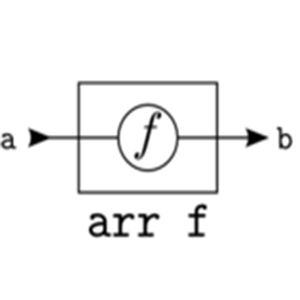
\includegraphics[width=0.4\textwidth]{Yampa-arr}
\caption[Yampa-arr]{Torna una función en SF.}
\label{fig:Yampa-arr}
\end{figure}

\begin{figure}[htbp!]
\centering
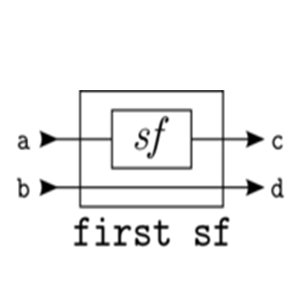
\includegraphics[width=0.4\textwidth]{Yampa-first}
\caption[Yampa-first]{Aplica un SF al primer elemento.}
\label{fig:Yampa-first}
\end{figure}

\begin{figure}[htbp!]
\centering
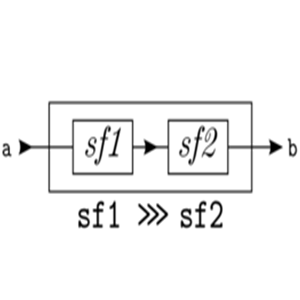
\includegraphics[width=0.4\textwidth]{Yampa-composition}
\caption[Yampa-composition]{Compone dos SF.}
\label{fig:Yampa-composition}
\end{figure}

\begin{figure}[htbp!]
\centering
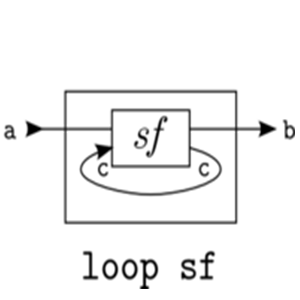
\includegraphics[width=0.4\textwidth]{Yampa-loop}
\caption[Yampa-loop]{Yampa loop}
\label{fig:Yampa-loop}
\end{figure}

Partiendo de estos combinadores se pueden derivar todos los combinadores más complejos usados por la librería \emph{Yampa}.

\subsection{Interruptores}

Los interruptores (\emph{Figura~\ref{fig:Yampa-switch}}) son elementos que permiten que las SF sean comportamientos capaces de cambiar en base a eventos externos además de cambiar con el tiempo. Los interruptores dan a las SF propiedades similares a la de una máquina de estados, donde los eventos causan una transición de un comportamiento a otro \cite{wiki:Yampa}.

\begin{figure}[htbp!]
\centering
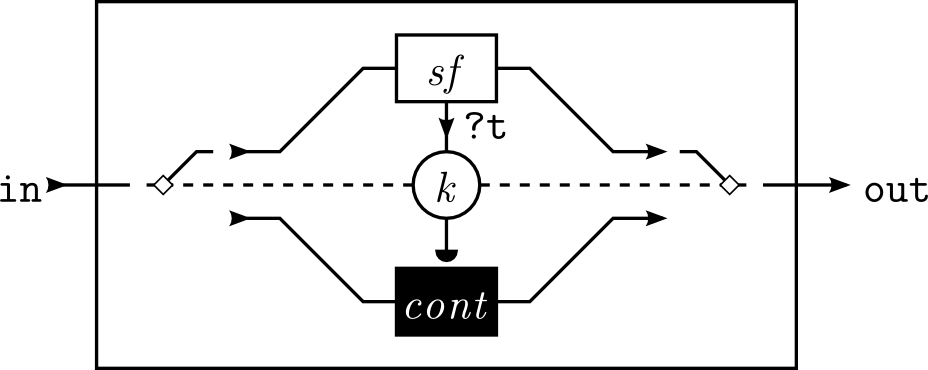
\includegraphics[width=0.4\textwidth]{Yampa-switch}
\caption[Yampa-switch]{Una SF cambia a una continuación al dispararse una condición k.}
\label{fig:Yampa-switch}
\end{figure}

\subsection{Ejemplo de uso de Yampa}

Las funciones de señal se pueden crear y manipular a través de la interfaz de Arrow. Por ejemplo, una transformación pura (a -> b) se convierte en una función de señal simplemente con arr de la clase Arrow. Aquí hay una función de señal que eleva a dos los valores que pasan a través de ella:

\begin{lstlisting}[frame=single]
square :: SF Double Double
square = arr (^2)
\end{lstlisting}

La función de utilidad \textbf{embed}  se puede usar para probar funciones de señal:

\begin{lstlisting}[frame=single]
embed square (1, [(0, Just 2), (1, Just 3)])
[1.0,4.0,9.0]
\end{lstlisting}

La firma de la función \textbf{embed} se ve así:

\begin{lstlisting}[frame=single]
embed :: SF a b -> (a, [(DTime, Maybe a)]) -> [b]
\end{lstlisting}

El primer argumento es la función de señal a muestrear. El segundo es una tupla que consiste en la entrada inicial a la función de señal y una lista de tiempos de muestra, posiblemente acompañada de un nuevo valor de entrada.

Un evento que contiene un valor de tipo a está representado por el Evento a:

\begin{lstlisting}[frame=single]
data Event a = Event a | NoEvent
\end{lstlisting}

Una fuente de evento es una función de señal con algún tipo SF a (Evento b). Algunos ejemplos de fuentes de eventos son los siguientes:

\begin{lstlisting}[frame=single]
never :: SF a (Event b)
now :: b -> SF a (Event b)
after :: Time -> b -> SF a (Event b)
\end{lstlisting}

Como el origen del evento es solo un SF normal, podríamos generar eventos con arr. Sin embargo, entonces debemos tener cuidado de que el evento se emita solo una vez: debido a que las uniones de señal son continuas, a menos que el evento se suprima en muestreos posteriores, podría ocurrir más de una vez.

Para reaccionar en eventos, necesitamos interruptores. El interruptor básico de una sola vez tiene el siguiente tipo:

\begin{lstlisting}[frame=single]
switch :: SF a (b, Event c) -- SF por defecto
          -> (c -> SF a b)   -- SF despues del evento
          -> SF a b
\end{lstlisting}

La siguiente señal produce la cadena foo durante los primeros 2 segundos, después de lo cual se dispara un evento y se produce bar:

\begin{lstlisting}[frame=single]
switchFooBar, switchFooBar' :: SF () String
switchFooBar = switch (constant "foo"&&& after 2 "bar") constant
switchFooBar' = dSwitch (constant "foo"&&& after 2 "bar") constant
\end{lstlisting}

La función dSwitch es idéntica a switch, excepto que, en el momento del evento, en la segunda el cambio es inmediato, en la primera el cambio se genera al siguiente muestreo.

\begin{lstlisting}[frame=single]
> embed switchFooBar ((), [(2, Nothing), (3, Nothing)])
["foo","bar","bar"]
> embed switchFooBar' ((), [(2, Nothing), (3, Nothing)])
["foo","foo","bar"]
\end{lstlisting}

Ejemplos mostrados en esta sección fueron creados por Samuli Thomasson, si el lector quiere profundizar en el uso de \emph{Yampa} leer ``Haskell High Performance Programming'' \cite{thomasson2016haskell} capítulo 13.

%!TEX root = ../thesis.tex

\chapter{Marco Metodológico}  %Title of the First Chapter
\label{capitulo3}

\ifpdf
    \graphicspath{{metodologia/Figs/Raster/}{metodologia/Figs/PDF/}{metodologia/Figs/}}
\else
    \graphicspath{{metodologia/Figs/Vector/}{metodologia/Figs/}}
\fi

A fin de mejorar la productividad en el desarrollo y la calidad del motor de juego, se hace uso de la metodología de desarrollo por prototipos. Esta  metodología se caracteriza por la construcción de un prototipo, el cual es evaluado y usado en un ciclo de retroalimentación, en donde se refinan los requisitos del software que se desarrollará \cite{mcconnell2004code}. Esta metodología permite probar la eficacia de diferentes algoritmos y la forma que debería tomar la interacción humano-máquina a través de diferentes prototipos, aspectos importantes para este proyecto, debido a que los algoritmos tradicionales para motores de juegos diseñados para lenguajes iterativos no son ideales para su uso en lenguajes funcionales.

\begin{figure}[!htbp!]
\centering
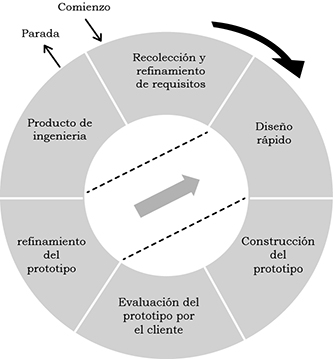
\includegraphics[width=0.5\textwidth]{metoPrototipo}
\caption[Metodología de desarrollo por prototipos]{Ciclo de desarrollo de una aplicación mediante la metodología de desarrollo por prototipos.}
\end{figure}

\section{Requisitos del sistema}

Ya que el objetivo de este proyecto es la creación de un motor de juego, los requisitos ideales que este debe suplir son los mismos que cualquier otro motor de juego, tener un motor gráfico para dibujar en pantalla, permitir a los programadores implementar la lógica de sus juegos, permitir a los artistas importar recursos al juego, un motor de física que resuelva colisiones entre objetos, entre otras características comunes antes mencionadas.

La diferencia que este proyecto debe necesariamente suplir, es funcionar en un lenguaje funcional, permitiendo a los programadores de los juegos trabajar con el mismo, y hacer el mayor uso posible de los beneficios que brinda la programación funcional para hacer que los juegos producidos sean lo más eficientes posible.

\section{Limitaciones del sistema}

Ya que crear un motor de juego con todas las características que poseen los motores profesionales es una labor colosal, este proyecto limitara las funcionalidades del programa final en lo mínimo requerido para poder producir juegos funcionales.

Las capacidades mínimas elegidas para poder producir juegos son, tener un  motor gráfico, poder cargar recursos para el motor gráfico, en este caso imágenes, shaders y mallados poligonales, y finalmente el motor lógico donde el programador implementará la funcionalidad del juego. Están serán tomadas como los requerimientos  mínimos que el programa final deberá de proveer como motor de juego, y serán usados como guía para la producción de los prototipos durante el desarrollo.

\section{Especificación de requisitos}

El programa final tendrá como usuario tres tipos de actores, que son los artistas, interesados principalmente en poder usar sus creaciones dentro del juego, los programadores, que implementan la lógica del juego usando el motor, y los jugadores, que si bien no interactúan directamente con el motor, lo hacen indirectamente a través de los juegos creados.

El principal caso de uso de los jugadores con el motor es el uso de los juegos, en ese aspecto el motor debe de encargarse de generar juego que transmitan correctamente las intenciones del jugador al sistema del juego. Para este proyecto este caso de uso se limitara a la entrada que el jugador genere vía el teclado, el ratón o modificaciones que este realice a la ventana del juego.

En cuanto a los artistas, el motor solo requiere tener la capacidad de cargar recursos para el motor gráfico.

El actor de mayor importancia para el programa final será el programador, este debe de tener la capacidad de implementar la lógica de su juego usando programación funcional, de preferencia con funciones puras. También se requerirá de un sistema que le permita correr funciones de E/S cuando se le sea necesario sin interferir con el flujo de cómputo de la lógica del juego, de preferencia en forma asíncrona. Finalmente el programador deberá de tener una manera de recibir y hacer cálculos con la entrada recibida del usuario y usar los recursos provistos por los artistas para dibujar en pantalla.

Adicionalmente de cubrir las necesidades de los actores, se espera que el motor haga el mayor uso posible de las facilidades ofrecidas por la programación funcional para hacer los que los juegos creados puedan hacer el mayor uso de los recursos del ordenador, especialmente en temas de paralelismo donde destaca la programación funcional.

\section{Arquitectura}

Los diferentes requerimientos del proyecto serán implementados en forma modular, para permitir que nuevos prototipos solo requieran la modificación de una sección del programa. Como el lenguaje de implementación \emph{Haskell} posee estándares para la construcción de paquetes y librerías \cite{wiki:WriteAHaskellProgram}, estos se utilizaran para la construcción del programa.

\section{Desarrollo}

Usando la metodología de desarrollo por prototipos, se implementará módulos que busquen satisfacer los requisitos del sistema junto con prototipos que hagan uso de estos módulos. A través de estos prototipos se decidirá la satisfacción de los requisitos y se entrará en un ciclo de corrección y ajuste.

\section{Documentación}

El presente documento servirá como el principal manual para el funcionamiento interno del programa. Para documentación que indique el uso y funcionamiento de las funciones públicas implementadas por el motor, se usara el estándar de comentarios de \emph{Haskell} para generar documentación con el programa Haddock.

%!TEX root = ../thesis.tex

\setcounter{secnumdepth}{4}

\chapter{Implementación}  %Title of the First Chapter
\label{capitulo4}

\graphicspath{{implementacion/Figs/Vector/}{implementacion/Figs/}}

Para el desarrollo de la aplicación se hizo uso del lenguaje \emph{Haskell} versión 8.0.2 y usando Cabal versión 1.24.2.0 como manejador de paquetes. Se escoge el lenguaje \emph{Haskell} sobre otros lenguajes funcionales por la consistencia que tiene este lenguaje a acatar de forma más estricta los conceptos asociados a la programación funcional y por ser un lenguaje compilado, lo que permite un mayor desempeño a tiempo de ejecución.

Dirigidos por la metodología de desarrollo por prototipos, se llevaron a cabo diversas iteraciones en las se expandió la funcionalidad del motor. Durante la primera iteración de trabajo se analizaron los métodos para graficar en \emph{Haskell} y se implementó el motor gráfico. En la segunda iteración se implementó el motor lógico y se establecieron los métodos con los cuales el programador puede implementar la lógica de su juego.  La tercera iteración se dedicó a la mejora del rendimiento del motor, añadiéndole la capacidad de correr los diferentes subsistemas en hilos de cómputo separados. La cuarta iteración, se añadió la capacidad para que el programador pueda correr funciones de E/S en forma asíncrona. En la quinta iteración se arreglaron desperfectos y se mejoró la interacción entre el motor y el programador según las experiencias obtenidas en los prototipos anteriores.

\section{Motor gráfico}

Este módulo debe contener las facilidades necesarias para el despliegue de gráficos en una ventana. La librería de despliegue gráfico seleccionada para el proyecto es OpenGL, que es una librería que interactúa con el GPU para brindar despliegue grafico acelerado por hardware. OpenGL tiene la ventaja de ser multiplataforma e independiente del sistema de ventanas y del sistema operativo en que corra la aplicación, permitiendo así a nuestra aplicación ser fácilmente portable entre diferentes dispositivos.

\subsection{Manejador de ventana}

La interfaz de OpenGL para \emph{Haskell} hace uso de la librería escrita en lenguaje c a través de la interfaz de funciones foráneas de \emph{Haskell}, haciendo necesario el uso de apuntadores e IO para poder interactuar con el contexto de OpenGL, siendo el objetivo de este módulo facilitar el despliegue gráfico, es importante hacer una librería que exponga una interfaz más funcional (de la misma forma en la que el monad IO oculta la naturaleza imperativa del mundo exterior) que sea más familiar a los usuarios de lenguajes funcionales y también que la librería provea de facilidades para cargar recursos multimedia al contexto de OpenGL así como controlar el proceso de despliegue gráfico.

El primer paso para usar OpenGL es la creación del contexto, para ello se ha elegido la librería GLUT, que es una librería de utilidades para aplicaciones que utilicen OpenGL, enfocándose primariamente en E/S a nivel de sistema operativo, operaciones como la creación y control de ventanas y entrada del teclado.

Trabajos realizados con GLUT se encuentran en el módulo \emph{EasyGLUT~\ref{EasyGLUT}}. La primera necesidad a la hora de usar GLUT está en definir callbacks para los diferentes eventos, entrada de mouse y teclado y cambios en el estado de la ventana. El motor gráfico provee funciones que inicializan una ventana GLUT (y consigo el contexto de OpenGL) y se definen diversos callbacks para el contexto de GLUT que procesan la entrada de la ventana y se acumula toda la entrada para ser procesada en el ciclo principal del programa.

Los callbacks definidos por el motor gráfico, permiten la detección de la entrada del usuario, que es almacenada en el tipo de dato \emph{MouseKey~\ref{MouseKey}}, que es una tupla que contiene un mapa del estado de las teclas y la posición del ratón. Usando esta información, el programador puede consultar en cualquier momento dado la entrada del jugador.

\begin{lstlisting}[label={MouseKey},frame=single,language=Haskell]
data KeyState = Down | Up | Pressed | Released deriving Show
data MouseState = FreeMouse GL.GLint GL.GLint | FixMouse GL.GLint GL.GLint
type MouseKey = (Map GLUT.Key KeyState,MouseState)
\end{lstlisting}

\subsubsection{GLUT como monad}

El motor gráfico también tiene la labor de manejar el ciclo principal de ejecución, y normalmente, al usar GLUT de forma convencional en \emph{Haskell}, este ciclo corre dentro del monad IO, permitiendo al usuario hacer cualquier cosa. Como la idea de un motor gráfico es que este se encargue de todos estos aspectos de E/S, se implementó el monad GLUT para sustituir al monad IO del ciclo principal del motor gráfico, y darle acceso al programador solo de las cosas que este pueda necesitar e impidiéndole alterar cosas que el motor gráfico controle.

Desde un punto de vista funcional, se puede considerar a GLUT como  un conjunto de cómputos que definen y controlan el estado de la ventana GLUT, así, estos cómputos pueden ser visto como un monad \cite{moggi1991notions} \cite{wiki:MonadsComputation} \cite{wiki:MonadsContainers}, que dentro de lenguajes funcionales facilitaría la interacción del usuario con la librería, ocultando apuntadores y demás detalles de comunicación con librería GLUT. De esta forma se introduce el monad GLUT que tiene las propiedades de poder ser consultado por eventos externos y entrada de dispositivos además de poder controlar una ventana de despliegue y un contexto de OpenGL.

\subsection{Carga de recursos}

Este módulo debe de proveer de herramientas para cargar recursos multimedia de formatos comunes. Esta sección tendrá un énfasis en imágenes y mallas poligonal que son los dos recursos multimedia con los cuales se puede hacer prototipos de juegos más rápidamente.

\subsubsection{Mallado poligonal}

El formato de archivos de mallado poligonal elegido para este proyecto es Wavefront .obj, que es un formato que guarda en forma simple información de geometría 3D en texto plano. Este es uno de los formatos más antiguos y es soportado por la gran mayoría de las herramientas de creación usadas por los artistas.

Ya que la información en un archivo Obj se guarda en texto plano, se crea un lexer y parser que puedan leer la información de un archivo. La información es guardada en el mismo formato en el tipo de dato Obj implementado en el módulo \emph{EasyGL.Obj~\ref{EasyGL.Obj}}.

\subsubsection{Imágenes}

Para la carga de imágenes se usa la librería JuicyPixels \cite{libreria:JuicyPixels} que soporta la lectura de imágenes en los formatos PNG, Bitmap, Jpeg, Radiance, Tiff y Gif. La carga de las imágenes se realiza en el módulo \emph{EasyGL.Material~\ref{EasyGL.Material}} al crear un material.

\subsection{Shaders}

El módulo \emph{EasyGL.Shader~\ref{EasyGL.Shader}} provee facilidades para cargar y compilar archivos de shaders a OpenGL. Todos los shaders compilados con esta librería poseerán atributos adicionales para recibir la posición del vértice, junto con su normal y coordenada de textura.

Este módulo ofrece funciones para cargar shaders de archivos y compilarlos. También implementa la función withShader que permite usar un shader en OpenGL de una manera funcional.

Adicionalmente, de la misma forma en que se realizó con GLUT,  se creó el monad Uniform que representa las acciones de cargar datos a los atributos de los shaders, que combinado con una clase Uniform, ayuda a garantizar que solo datos que puedan ser aceptados por el GPU sean cargados a este. Este monad premite la creación de la función withShaderSafe que permite usar un shader en forma segura ya que todo el pasaje de información al shader se hace por el monad Uniform.

\subsection{Materiales}

En el módulo \emph{EasyGL.Material~\ref{EasyGL.Material}} define el tipo de dato Material que contiene referencia a un shader ya compilado y a texturas que ya han sido cargadas a OpenGL. Este módulo solo ofrece la facilidad de cargar automáticamente texturas al shader contenido en el material.

\subsection{Cámara}

Se necesitan facilidades para el controlar los elementos a dibujar así como la perspectiva a usarse en los dibujos, este módulo debe ser capaz de utilizar los recursos cargados en otros módulos y producir imágenes en la ventana del juego. El módulo \emph{EasyGL.Camera~\ref{EasyGL.Camera}} ofrece una abstracción de cámara fácil de usar, que oculta las dificultades de configurar la visión en OpenGL así como la manipulación de matrices de transformación que ellos implican.

\subsection{Despliegue gráfico}

Para poder hacer uso de los mallados poligonales se debe primero cargar la información de los mismos al GPU. OpenGL hace uso de objetos conocidos como Vertex Array Object (VAO) y Vertex Buffer Object (VBO) como medios para almacenar información en el GPU y dibujar un objeto en pantalla de forma rápida y eficiente. Estos objetos pueden ser usados para cargar información de la posición de los vértices, la coordenada de las texturas y las normales del objeto, que es información que podemos obtener de los archivos Obj.

Ya que la información que se almacena en VAO's y en VBO's se ordena en forma diferente a la información almacenada en los archivos Obj, se implementó en el módulo \emph{EasyGL.IndexedModel~\ref{EasyGL.IndexedModel}} el tipo de dato IndexedModel, que almacena la información de un mallado (vertices, coordenadas de texturas y normales) en el orden y formato que se requiere para crear VAO's y VBO's. Uan gran ventaja que provee el dato IndexedModel, es que sirve como un intermediario para cargar información al GPU, y cualquier módulo que se agregue al proyecto para cargar algún formato de objeto poligonal al sistema, solo debe de implementar un método que convierta la información en un IndexedModel. Para cargar al GPU y dibujar en pantalla un IndexedModel, se usan las funciones implementadas en el modulo \emph{EasyGL.Entity~\ref{EasyGL.Entity}}.

Para cargar la información de los archivos Obj a OpenGL, se implementa el módulo \\\emph{EasyGL.Obj.Obj2IM~\ref{EasyGL.Obj.Obj2IM}}, que lee el archivo y transforma la información en un IndexedModel.

%\subsection{Extras}

%\subsubsection{Utils}
%\subsubsection{mem}

\section{Motor lógico}

Esta sección del programa se encargara de mantener y actualizar a los diferentes objetos del juego a medida que transcurre el tiempo. Este módulo debe de proveer al usuario las herramientas necesarias para implementar la lógica de su juego e inicializarlo al ser invocado. Para aprovechar las ventajas de la programación funcional la actualización de objetos debe de ejecutarse de una forma pura.

Permitir que el usuario implemente la lógica de su juego es de vital importancia para todo motor de juego, y como ya se mencionó en la \emph{sección~\ref{sec:MTlogica}}, los motores de juegos modernos emplean el patrón sistema entidad-componente, este patrón de diseño en su implementación depende en gran medida de la existencia de un estado mutable, la lógica creada por el usuario inevitablemente tiene que modificar componentes de una o más entidades para poder así generar cambios en el estado del juego. Sistemas implementados usando este patrón además requieren complejos sistemas para llevar a cabo la comunicación entre diversos subsistemas, y además, como muestra Jeff Andrews \cite{andrews2009designing}, la complejidad se hace mucho mayor cuando se quiere que estos sistemas corran de forma concurrente para hacer mejor use de procesadores modernos.

La implementación de un sistema que haga uso del patrón sistema entidad-componente en un lenguaje funcional como \emph{Haskell} es posible si se hace que todas las entidades se referencien con apuntadores y solo sean accesibles dentro del monad IO, semejante implementación podría dar los mismos resultados que en lenguajes imperativos, pero se incurriría en los mismos problemas sufridos en estos lenguajes además de no aprovechar ninguna de las ventajas que ofrece la programación funcional como las funciones puras.

La programación funcional reactiva es un paradigma de programación que nos permite sustituir al modelo sistema entidad-componente. Para este proyecto se ha decidido usar la librería \emph{Yampa}, que implementa \emph{FRP} y puede ser usado para mantener y actualizar una colección de entidades en forma pura.

\subsection{Tipos de datos}

Siguiendo el ejemplo de visto en “The Yampa Arcade” \cite{Courtney2003b}, podemos representar los objetos del juego como una SF que recibe como entrada el estado previo del juego y la entrada del jugador y retorna el nuevo estado del objeto así como la información necesaria para interactuar con los subsistemas del motor. Así un objeto tiene la forma:

\begin{lstlisting}[label={ObjDef1},frame=single,language=Haskell]
type Object = SF ObjInput ObjOutput
\end{lstlisting}

Esta abstracción nos permite distinguir los objetos de nuestro juego de otras SF. \emph{ObjInput} y \emph{ObjOutput} deben de ser definidos tomando en consideración que el usuario debe de poder usar su propio tipo de dato para representar el estado del juego y otro tipo de dato que represente los eventos que este quiera generar por su cuenta.

\begin{lstlisting}[label={ObjInputDef},frame=single,language=Haskell]
data ObjInput state eventType = ObjInput {
  oiEvents :: Event eventType,
  oiGameInput :: GameInput,
  oiPastFrame :: IL state
}
\end{lstlisting}

\emph{ObjInput} es definido como un tipo de dato que contiene la entrada del juego representada en el tipo GameInput, eventos que este objeto reciba y la colección de los objetos en el frame anterior del juego.

\begin{lstlisting}[label={ObjOutputDef},frame=single,language=Haskell]
data ObjOutput state eventType = ObjOutput {
  ooObjState :: !state,
  ooRenderer :: Maybe (ResourceIdentifier,Transform,Uniform ()),
  ooKillReq :: Event (),
  ooSpawnReq :: Event [Object state eventType],
  ooWorldReq :: [IOReq eventType],
  ooWorldSpawn :: [IO ()],
  ooUIReq :: [UIActions]
}
\end{lstlisting}

Cada registro del tipo \emph{ObjOutput} almacena:

\begin{itemize}
\item ooObjState: el estado de salida del objeto. Contiene la información relevante a la lógica del juego y es el único campo visible por otros objetos. Es estricto para garantizar que no existan fugas de memoria.
\item ooRenderer: este campo permite al objeto indicar al motor gráfico que dibujar. Si este campo contiene un Nothing entonces nada será dibujado en pantalla, de ser un Just, este contendrá una tupla con el id del mesh a usar, la posición en el espacio y los datos a enviar al shader.
\item ooKillReq: indica al sistema si se debe o no destruir el objeto.
\item ooSpawnReq: indica al sistema los nuevos objetos que se quiere crear.
\item ooWorldReq: hace al sistema iniciar una nueva operación de E/S cuyo resultado será de tipo \emph{eventType}. Este resultado será luego devuelto al objeto vía \emph{ObjInput} cuando esté disponible.
\item ooWorldSpawn: crea una nueva operación de E/S cuyo resultado no importa.
\item ooUIReq: permite interactuar con el manejador de ventana (GLUT en este caso).
\end{itemize}

Con la entrada y salida de nuestros objetos definidos, la nueva firma del tipo objeto pasa a ser:

\begin{lstlisting}[label={ObjDef2},frame=single,language=Haskell]
type Object outState eventType = SF
    (ObjInput outState eventType)
    (ObjOutput outState eventType)
\end{lstlisting}

Ahora que se ha definido el tipo de datos para los objetos del juego, es necesario poder crear una colección de estos objetos, esta colección requiere que cada objeto pueda ser identificado de manera única. En el módulo \emph{Val.Strict.IL~\ref{Val.Strict.IL}} se implementa el tipo de dato \emph{IL} (Identity List), \emph{IL} se define como:

\begin{lstlisting}[frame=single,language=Haskell]
type ILKey = Integer
data IL a = IL {
    ilNext :: ILKey,
    ilAssocs :: Map ILKey a
  }
\end{lstlisting}

El tipo \emph{IL} almacena los objetos en un mapa de la librería \emph{Data.Map}, que este posee muy buen tiempo para insertar, eliminar, consultar y recorrer, de usar un arreglo el tiempo para la inserción, la eliminación y la consulta serían mayores por requerir que los objetos sean identificables. Cada objeto es identificado con un \emph{ILKey} al momento de ser insertado.

Para hacer su uso lo más conveniente posible, el modulo \emph{Val.Strict.IL~\ref{Val.Strict.IL}} define múltiples funciones de consulta y modificación con \emph{IL}, además de incluir a \emph{IL} en las clases \emph{Functor}, \emph{Foldable}, \emph{Traversable} y \emph{NFData}.

\subsection{Escenas}
\label{sec:Escenas}

Para crear una escena de juego, se requiere primero una forma de actualizar la colección de objetos, para ellos se hace uso del dpSwitch de la librería \emph{Yampa}. Este suiche se caracteriza por manejar colecciones dinámicas de objetos, en el módulo \emph{Val.Strict.Scene~\ref{Val.Strict.Scene}} se hace uso de este suiche para crear la SF “sceneSF” que tiene la firma:

\begin{lstlisting}[frame=single,language=Haskell]
SF
  (GameInput, IL (ObjOutput s et), IL (Event et))
  (IL (ObjOutput s et))
\end{lstlisting}

La SF sceneSF recibe como entrada el estado de la ventana y entrada del usuario, el estado de los objetos en el frame anterior y eventos que deban ser enviados a objetos específicos, y retorna como resultado los objetos actualizados.

Con sceneSF es posible ahora implementar el ciclo principal del juego, el módulo \emph{Val.Strict.Scene \ref{Val.Strict.Scene}} implementa la función initScene, que dado la información de los recursos a usar, una SF que controle una cámara y una colección inicial de objetos, carga todos los recursos al sistema e inicia el ciclo principal.

La función initScene inicia la escena del juego creando tres hilos de cómputo encargados de tareas específicas, en la \emph{Figura~\ref{fig:ciclo_de_juego}} se puede apreciar el flujo de los datos entre los hilos. Cada hilo esta e
encargado de:

\begin{itemize}
\item Hilo 1, hilo lógico: Este hilo se caracteriza por actualizar la colección de objetos cada frame, este hilo inicia recibiendo la entrada del usuario del hilo 2 y el retorno de las funciones asíncronas generadas por los objetos manejados por el hilo 3. Con estos dos datos se actualizan los objetos en base al tiempo transcurrido y la salida de ellos es transmitida a los otros hilos.
\item Hilo 2, hilo de despliegue: Este hilo maneja el contexto de OpenGL y GLUT, inicia enviando la entrada del usuario al hilo 1 y recibe la salida de los objetos generados en el hilo 1. Con esta salida se puede generar el despliegue de gráficos.
\item Hilo 3, hilo de E/S: Este hilo existe para que los objetos del juego puedan ejecutar funciones de E/S de manera asíncrona. Este hilo mantiene una lista de todas las funciones asíncronas en corrida. Este hilo inicia evaluando la culminación de alguna función y enviando los resultados al hilo 1, luego recibe la salida del hilo 1 y corre cualquier nueva función asíncrona que los objetos soliciten.
\end{itemize}

\begin{figure}[!htbp!]
\centering
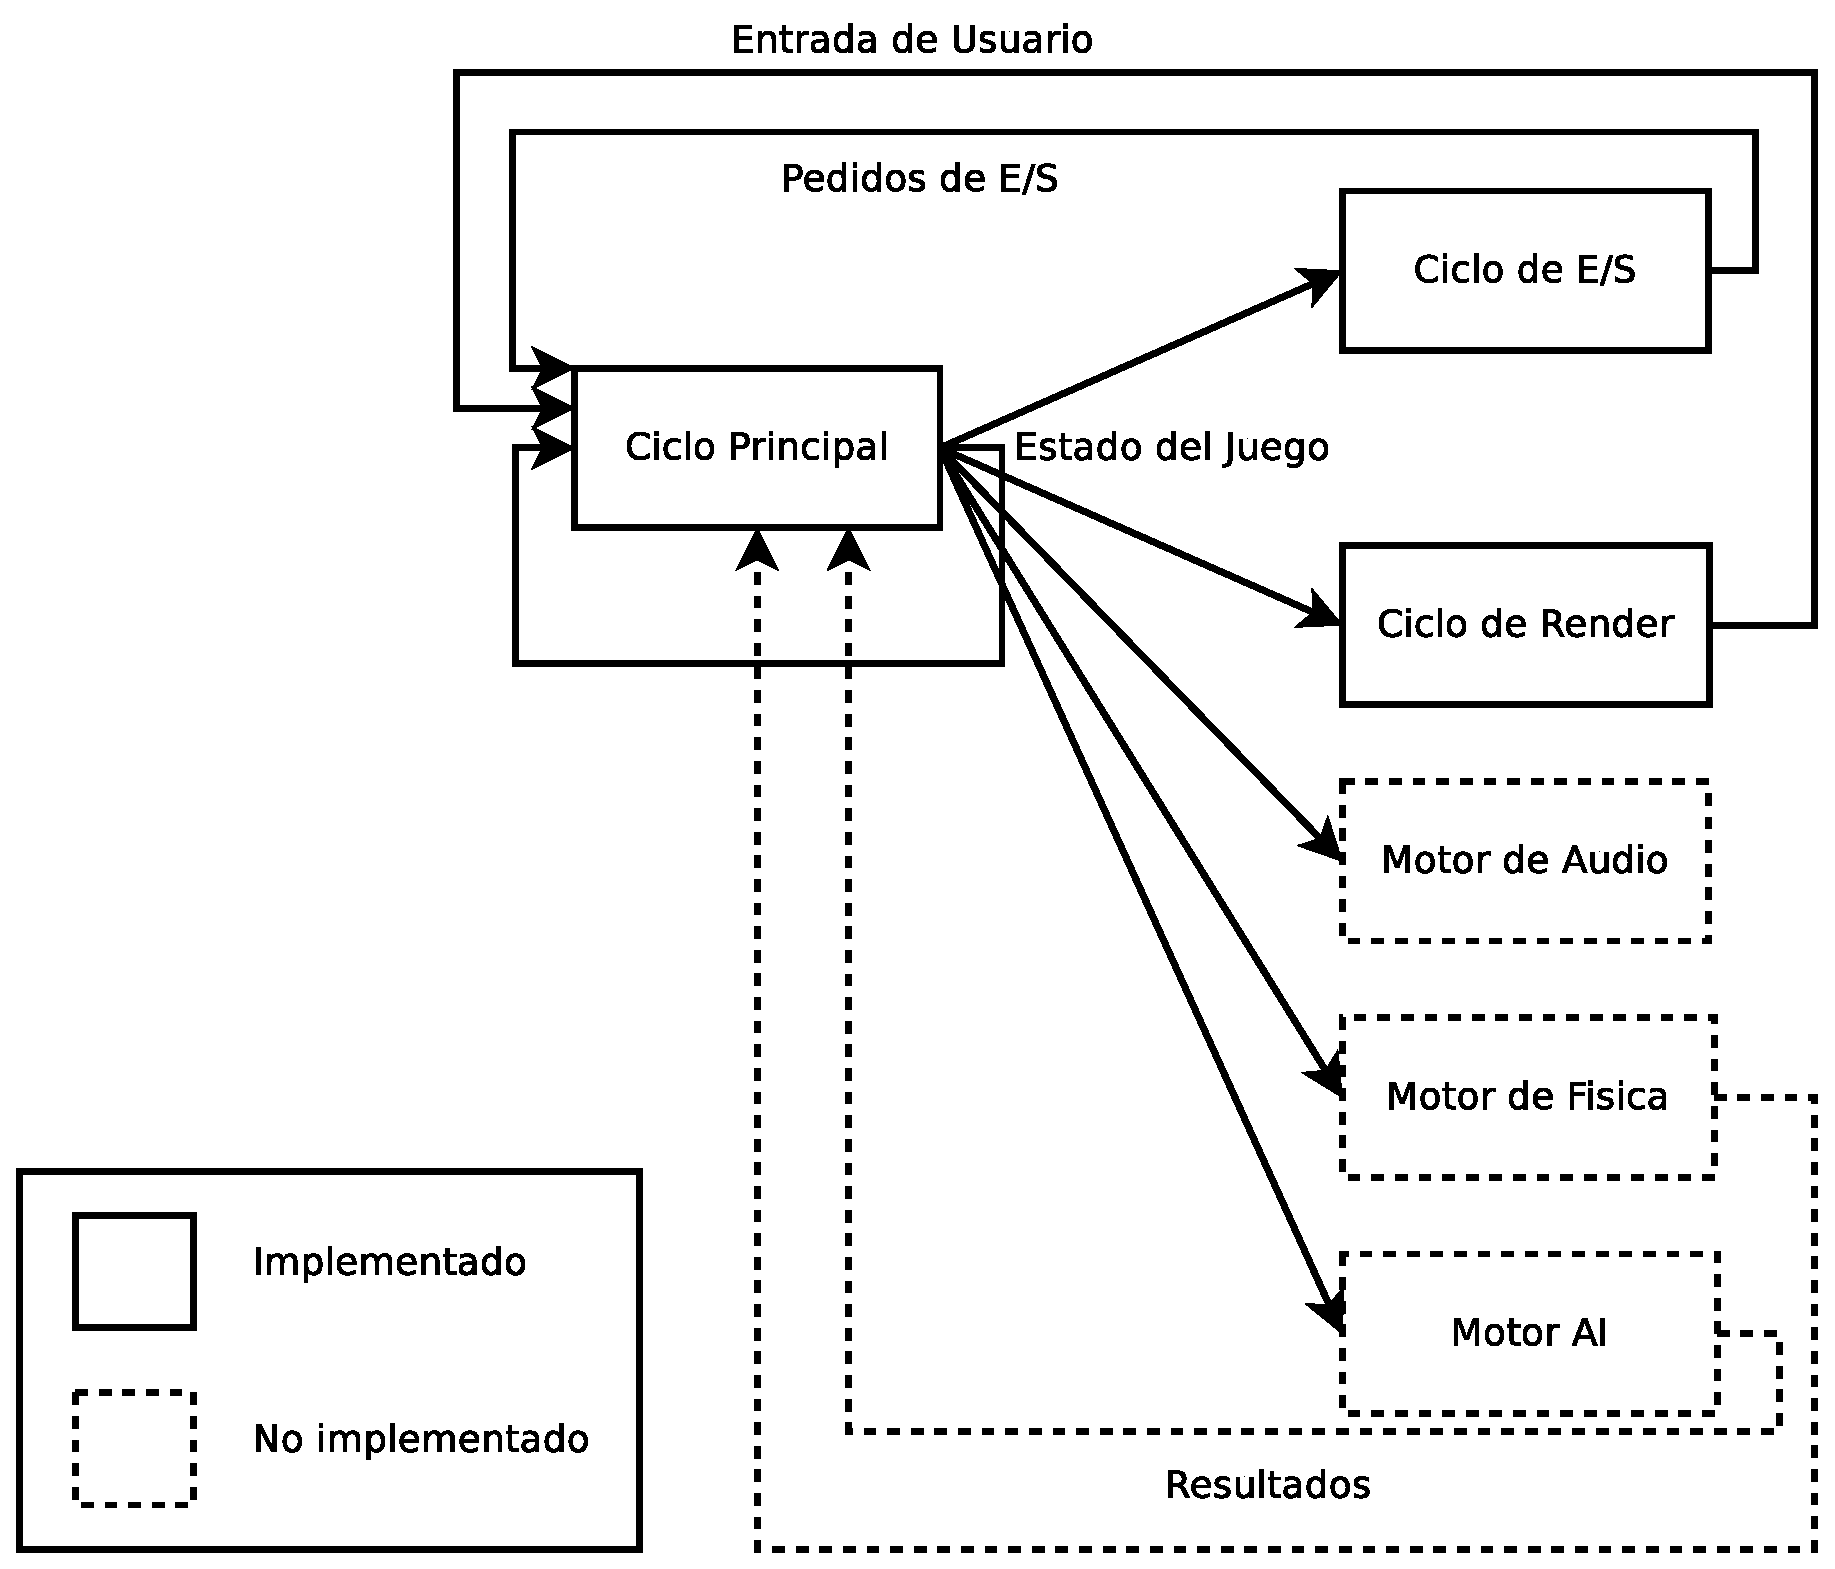
\includegraphics[width=1.0\textwidth]{ciclo_de_juego}
\caption[Ciclo de juego]{Esta figura muestra los diferentes hilos que corren en una escena de juego y a donde se envían los resultados de cada unos de ellos.}
\label{fig:ciclo_de_juego}
\end{figure}

Como cada hilo solo requiere de una referencia a los resultados de los objetos del juego para correr, que son valores inmutables y por lo tanto no pueden afectar a otros hilos, se puede añadir otros hilos nuevos con otro tipo de funcionalidad como sonido, networking, inteligencia artificial, entre otros, sin alterar el funcionamiento ya implementado y sin modificar la lógica actual.

La comunicación entre los diferentes hilos se logra con el uso de \emph{MVar}, que son apuntadores especiales de \emph{Haskell} que tienen la propiedad de funcionar como semáforos, haciendo que los hilos solo puedan enviar información a otros una vez estos estén listos para recibirla. El uso de estas \emph{MVar} causa, en la implementación actual, que todos los hilos se sincronicen al más lento.

El módulo \emph{Val.Strict.Scene~\ref{Val.Strict.Scene}} ademas aprovecha el hecho de que el tipo \emph{IL} implemente la clase \emph{Traversable}, con esta clase se puede usar la librería \emph{Control.Parallel.Strategies} de \emph{Haskell} para que el calculo de los diferentes objetos del juego se realice en forma concurrente manejado por el runtime environment de \emph{Haskell}, permitiendo que los cálculos realizados en el hilo lógico puedan realizare en más de un procesador. Para poder usar esta versión del hilo lógico, el usuario solo debe cambiar la llamada de la función initScene por la función initScenePar implementada en el mismo módulo.

\subsection{Utilidades}

Ya que \emph{FRP} es un concepto complicado (de aprender a usar), puede resultar ser una barrera para usar el motor de juego, por ello se ha creado en el módulo \emph{Val.Strict.Util~\ref{Val.Strict.Util}} la función makeSF que tiene la firma:

\begin{lstlisting}[frame=single,language=Haskell]
makeSF :: a
  -> (a -> ObjInput b c -> (a,ObjOutput b c))
  -> Object b c
\end{lstlisting}

Con la función makeSF el usuario puede crear un objeto de juego sin usar \emph{FRP} o la librería \emph{Yampa}. Esta función toma como primer argumento un estado inicial y de segundo una función que toma ese estado, una entrada de objeto y retorna el estado actualizado y una salida de objetos.

Sin embargo esta forma de crear objetos de juego carece de la capacidad de cambiar comportamiento a medida que corre el programa que posee \emph{FRP}, un objeto creado con esta función solo podrá tener el comportamiento de la función dada en el segundo argumento. La única manera de cambiar el comportamiento es creando un objeto nuevo y destruir el viejo.

%!TEX root = ../thesis.tex

\chapter{Resultados}
\label{capitulo5}

\ifpdf
    \graphicspath{{resultados/Figs/Raster/}{resultados/Figs/PDF/}{resultados/Figs/}}
\else
    \graphicspath{{resultados/Figs/Vector/}{resultados/Figs/}}
\fi

El proyecto logró producir una herramienta que permite la creación de juegos en lenguaje Haskell. Para poder comprobar su funcionalidad y desempeño se hace uso de programas de ejemplo creados usando la herramienta.

\section{Ejemplos del motor gráfico}

Para la prueba del motor gráfico se crearon varios programas de prueba con escenas diferentes donde se pudiese apreciar la funcionalidad del motor gráfico. Uno de los ejemplos más sencillos es un programa que dibuja en pantalla el armadillo de Stanford usando su normal como textura, ver Figura~\ref{fig:Ejemplo_1}. Este programa no tiene ninguna clase de interacción. Se puede ver el programa en la sección de código Ejemplo1~\ref{Ejemplo1}, el código requerido para este programa es sencillo y corto gracias al motor. Otro ejemplo, Figura~\ref{fig:Ejemplo_2}, muestra una escena más compleja usand el motor gráfico.

\begin{figure}[!ht!]
\centering
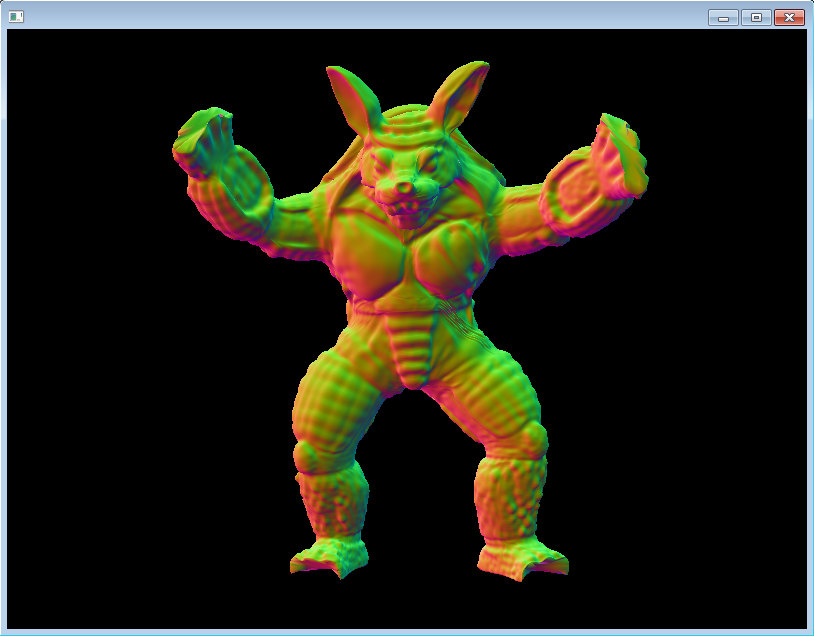
\includegraphics[width=0.6\textwidth]{armadillo}
\caption[Ejemplo 1]{El armadillo de Stanford dibujado usando su normal como color.}
\label{fig:Ejemplo_1}
\end{figure}

\begin{figure}[!ht!]
\centering
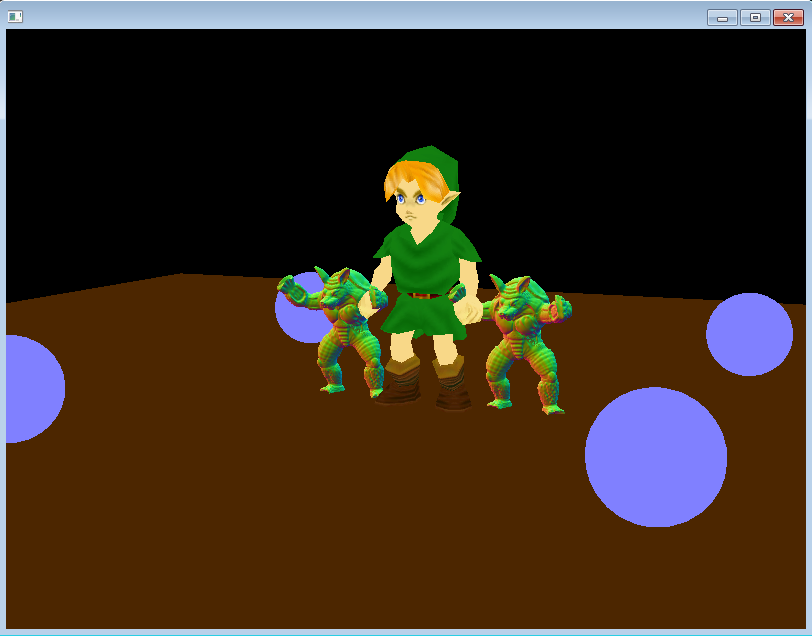
\includegraphics[width=0.6\textwidth]{link}
\caption[Ejemplo 2]{Una escena mas compleja usando el motor gráfico.}
\label{fig:Ejemplo_2}
\end{figure}

\section{Ejemplo motor de juego}

El motor de juego se prueba mediante un programa que crea un número de esferas que se mueven en alguna dirección e invierten la dirección en la que se mueven cuando colisionan con otra esfera o llegan al límite de un área predefinida. Este ejemplo se puede encontrar en la sección de código Ejemplo2~\ref{Ejemplo2}.

Para este ejemplo se observa los FPS (frames per second) del programa con diferente cantidad de esferas y permitiendo al RTE de haskell correr con una cantidad diferente de hilos máximos. Esta prueba permitirá observar el rendimiento y el uso de paralelismo del motor de juego en diversas situaciones.

\begin{table}
\begin{tabular}{ | l | c | c | c | c | }
 \hline
 FPS & 1 hilo &2 hilos&3 hilos&4 hilos\\
 \hline
 5 esferas & 1550	& 1650	& 1820	& 1780 \\ \hline
 10 esferas & 1350	& 1480	& 1550	& 1520 \\ \hline
 50 esferas & 430	& 520	& 650	& 620 \\ \hline
 100 esferas & 212	& 270	& 350	& 340 \\ \hline
 200 esferas & 100	& 150	& 160	& 160 \\ \hline
 400 esferas & 42	& 68	& 72	& 72 \\ \hline
 600 esferas & 27	& 40	& 44	& 44 \\
 \hline
\end{tabular}
\caption{FPS en corridas de Ejemplo 2.}
\label{table:Ejemplo2}
\end{table}

En la tabla~\ref{table:Ejemplo2} se observa, como era de esperarse, una disminución de los FPS a medida que se aumenta el número de entidades en la escena. Pero gracias al uso de paralelismo del motor, el uso de hilos adicionales permite aumentar el número de FPS por cantidad de entidades. Los datos muestran que el programa corre a mayor velocidad cuando se utilizan tres hilos de cómputo, en especial en los casos con pocas entidades.

En los casos con pocas entidades, la caída en FPS puede atribuirse al costo incurrido en crear y destruir hilos siendo mayor a la ganancia de procesar las entidades en hilos separados. Sin embargo, cuando se aumenta el número de entidades, los FPS con tres y cuatro hilos se hacen iguales en lugar de aumentar, en la sección ~\ref{sec:Escenas} se establece que el hilo lógico usa la librería Control.Parallel.Strategies para realizar la actualización de las entidades en paralelo, el motor de juego posee, en la implementación actual, tres hilos que siempre se encuentran activos, cualquier otro hilo es creado en base a demanda. Ello significa que al usar tres hilos el RTE de Haskell corra la actualización de las entidades en el hilo asignado al hilo lógico, pero al haber cuatro, el RTE puede estar incurriendo en un problema en el que administrar que tareas asignar a este hilo disponible sea más caro que la tarea siendo asignada al hilo. La otra posible causa de no aprovecharse el cuarto hilo yace en que la estrategia usada de la librería Control.Parallel.Strategies no esté llevando los objetos a forma normal, en haskell eso significa que un cómputo este totalmente computado y no sea una promesa, que podría ser resuelto cambiando de estrategia e implementando la clase NFData para el tipo de dato ObjOutput.

Este ejemplo muestra que el uso de hilos en el motor provee de mayor rendimiento a los juegos creados sin aumentar la complejidad del motor. Es recomendable para cualquier funcionalidad adicional que se agregue al motor, el implementarse un hilo separado que solo dependa del estado del juego.

\begin{figure}[!ht!]
\centering
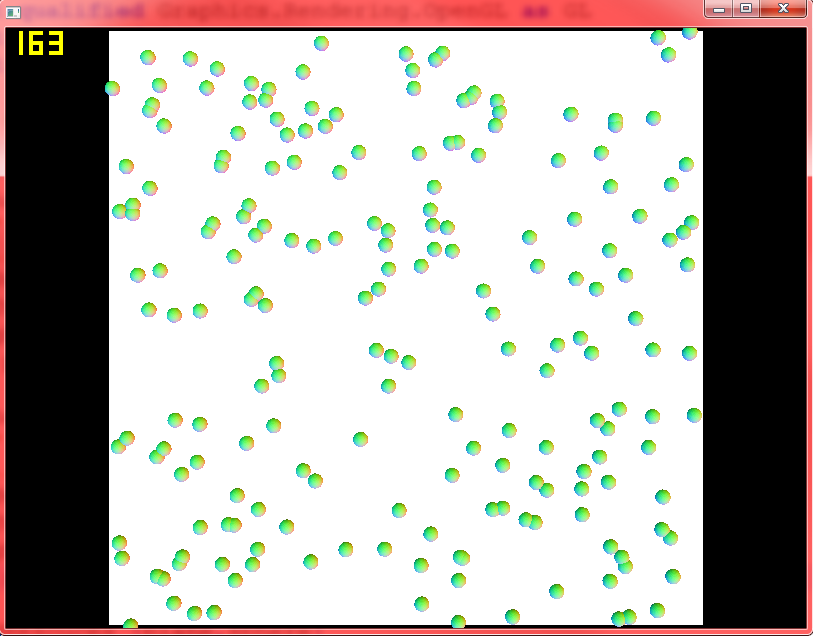
\includegraphics[width=0.8\textwidth]{sceenshot2}
\caption[Ejemplo 3]{200 esferas.}
\label{fig:Ejemplo_3}
\end{figure}

Otros ejemplos fueron creados para probar el motor de juego, algunos de esos ejemplos usan algoritmos de inteligencia artificial para tener entidades capaces de interactuar con el jugador y donde el jugador puede controlar una entidad, otro ejemplo permite simplemente navegar por un espacio virtual. Sin embargo ya que el rendimiento observado en los otros ejemplos es similar al Ejemplo2~\ref{Ejemplo2} y que el código de estos ejemplos es considerablemente largo, no se hace mención detallada de estos otros ejemplos.

%\section{Sobre GLUT y OpenGL}

%El uso de monads para expresar las operaciones relativas a GLUT resulta como una manera más cómoda y segura para interactuar con la librería según la experiencia adquirida en el uso del monad. Esta experiencia es consistente con un caso similar en el cual Facebook uso monads y Aplicative (clase de haskell) para expresar cómputos paralelos en sus reglas de filtrado de spam, que gracias a la notación de monad de haskell hace el código más limpio y seguro \cite{marlow2014there} \cite{Facebook:Fighting} \cite{Facebook:sourcing}.

%De la misma forma en la que se logró crear un monad para GLUT,  debe ser posible crear uno similar para OpenGL, que al igual que GLUT comparte muchas similitudes en funcionamiento. Actualmente, la implementación actual no monádica de OpenGL fuerza a que todas las llamadas a funciones de OpenGL deban realizarse en monad IO, lo cual es considerado peligroso ya que cualquier tipo de código puede ser ejecutado en dicho entorno, y al OpenGL tener que correr en IO, es necesario tener que incluir al monad GLUT en la clase MonadIO (que permite a cualquier monad correr IO) para poder correr código OpenGL en el ciclo de ejecución de GLUT, arruinando en cierta medida la idea de seguridad que se esperaba para el monad GLUT.

%De poder implementarse un monad para OpenGL, se podría eliminar toda posibilidad de hacer IO en las secciones de código que pertenezcan a GLUT y a OpenGL, lo cual, si bien puede parecer restrictivo, ayudaría a que el monad garantice consistencia en los contextos de ambas librerías \cite{hughes2000generalising}.

%La razón principal por la cual un monad no fue implementado para OpenGL es, primero, la librería OpenGL es proporcionalmente más grande y compleja que GLUT. Segundo, en OpenGL se pueden crear objetos únicos de esta librería (ejemplo: VOBs) y su administración y almacenamiento es un tema de discusión, ya que de ser dejado al usuario se rompe la idea de que un monad OpenGL maneje todo el contexto de OpenGL, y dejado como responsabilidad de un posible monad, es difícil dar con una interfaz que resulte cómoda y llamativa para el usuario.

%!TEX root = ../thesis.tex

\chapter{Conclusiones}
\label{capitulo6}

Con la realización de este trabajo se logró la creación de una herramienta que simplifica la creación de juegos en un entorno de programación funcional. La herramienta creada permite el despliegue grafico de objetos, el manejo de la entrada del usuario, pedidos de E/S y la actualización, de forma pura, entidades de juego que interactúan entre sí que conforman la escena del juego.

Un avance importante que provee la herramienta creada al conocimiento de motores de juego está en la habilidad de optimizar para el paralelismo. Como la herramienta requiere que el usuario programe las entidades del juego en forma pura, es posible ejecutar el código del usuario en un orden arbitrario sabiendo que este no interactúa con otros elementos y que su resultado no será alterado. Esta flexibilidad permite procesar la actualización de cada entidad en hilos de cómputo separados. Adicionalmente, como la información de las entidades es inmutable, se puede compartir con otros hilos de cómputo que usen la información para operaciones de entrada y salida (como graficar) de forma segura.

Esta misma pureza en la programación de las entidades, combinada con un sistema de tipos estricto como el de haskell, permite que la herramienta sea útil para detectar errores de forma temprana en el código de nuestros juegos.

La estructura del motor permite que nueva funcionalidad  sea fácilmente añadida, solo se tiene que pedir a las entidades que su salida provea la interfaz requerida por la nueva funcionalidad. Cualquier nueva funcionalidad, como por ejemplo un motor de física, podría fácilmente ser añadido a la herramienta para que corra en un hilo de computo independiente, ya que esta solo requeriría un apuntador a la información de las entidades y esta información es inmutable, permitiendo al motor de física realizar su función sin tener que cambiar otros sistemas para poder añadirlo.

La experiencia con el motor muestra la conveniencia de usar FRP como máquinas de estado, comparando con una implementación imperativa, como la propuesta en el libro “Artificial intelligence for games” \cite{millington2016artificial}, FRP resulta mucho más modular y re utilizable mientras que esconde la transiciones entre los estados.

También es de notar que durante la creación de juego de prueba hechos usando la herramienta, se realizaron múltiples cambios en la interfaz que permite la interacción de las entidades del juego con los diferentes sistemas de la herramienta, esto es debido a que en ciertas circunstancias ciertas formas de hacer las cosas resulta más cómodo, y con una herramienta tan joven como esta, solo su uso continuo proveerá una mejor visión de los cambios requeridos para hacer su uso más placentero a cualquier posible usuario en un futuro, esta es una herramienta que todavía posee espacio para mejorar y ser expandida.


%%!TEX root = ../thesis.tex

\chapter{Código}

\lstinputlisting[label={EasyGL},caption={EasyGL.hs},language=Haskell]{./code/src/EasyGL.hs}
\lstinputlisting[label={EasyGLUT},caption={EasyGLUT.hs},language=Haskell]{./code/src/EasyGLUT.hs}
\lstinputlisting[label={EasyGL.Camera},caption={Camera.hs},language=Haskell]{./code/src/EasyGL/Camera.hs}
\lstinputlisting[label={EasyGL.EasyMem},caption={EasyMem.hs},language=Haskell]{./code/src/EasyGL/EasyMem.hs}
\lstinputlisting[label={EasyGL.Entity},caption={Entity.hs},language=Haskell]{./code/src/EasyGL/Entity.hs}
\lstinputlisting[label={EasyGL.IndexedModel},caption={IndexedModel.hs},language=Haskell]{./code/src/EasyGL/IndexedModel.hs}
\lstinputlisting[label={EasyGL.Material},caption={Material.hs},language=Haskell]{./code/src/EasyGL/Material.hs}
\lstinputlisting[label={EasyGL.Obj},caption={Obj.hs},language=Haskell]{./code/src/EasyGL/Obj.hs}
\lstinputlisting[label={EasyGL.Obj.Grammar},caption={Grammar.y},language=Haskell]{./code/src/EasyGL/Obj/Grammar.y}
\lstinputlisting[label={EasyGL.Obj.Obj2IM},caption={Obj2IM.hs},language=Haskell]{./code/src/EasyGL/Obj/Obj2IM.hs}
\lstinputlisting[label={EasyGL.ObjData},caption={ObjData.hs},language=Haskell]{./code/src/EasyGL/Obj/ObjData.hs}
\lstinputlisting[label={EasyGL.Obj.Tokens},caption={Tokens.x},language=Haskell]{./code/src/EasyGL/Obj/Tokens.x}
\lstinputlisting[label={EasyGL.Shader},caption={Shader.hs},language=Haskell]{./code/src/EasyGL/Shader.hs}
\lstinputlisting[label={EasyGL.Texture},caption={Texture.hs},language=Haskell]{./code/src/EasyGL/Texture.hs}
\lstinputlisting[label={EasyGL.Util},caption={Util.hs},language=Haskell]{./code/src/EasyGL/Util.hs}

\lstinputlisting[label={Val.Strict},caption={EasyGL.hs},language=Haskell]{./code/src/Val/Strict.hs}
\lstinputlisting[label={Val.Strict.Data},caption={EasyGL.hs},language=Haskell]{./code/src/Val/Strict/Data.hs}
\lstinputlisting[label={Val.Strict.Events},caption={EasyGL.hs},language=Haskell]{./code/src/Val/Strict/Events.hs}
\lstinputlisting[label={Val.Strict.IL},caption={EasyGL.hs},language=Haskell]{./code/src/Val/Strict/IL.hs}
\lstinputlisting[label={Val.Strict.Scene},caption={EasyGL.hs},language=Haskell]{./code/src/Val/Strict/Scene.hs}
\lstinputlisting[label={Val.Strict.UI},caption={EasyGL.hs},language=Haskell]{./code/src/Val/Strict/UI.hs}
\lstinputlisting[label={Val.Strict.Util},caption={EasyGL.hs},language=Haskell]{./code/src/Val/Strict/Util.hs}
\lstinputlisting[label={Val.Strict.Scene.Resources},caption={EasyGL.hs},language=Haskell]{./code/src/Val/Strict/Scene/Resources.hs}

\begin{lstlisting}[label={Ejemplo1},caption={Ejemplo - Mostrando armadillo},language=Haskell]
import EasyGL
import EasyGLUT
import System.Exit
import System.IO (stderr)
import Control.Monad.IO.Class (MonadIO,liftIO)
import qualified Graphics.Rendering.OpenGL as GL

armadillo :: Shader -> IO (Material,Entity)
armadillo myShader = do
  m <- makeMaterial myShader []
  case m of
    Left s -> putStrLn s >> exitFailure
    Right mat -> do
      e <- readObj2Ent "./armadillo.obj"
      return (mat,e)

main = do
	-- se inicializa el contexto de OpenGL y GLUT.
  initOpenGLEnvironment 800 600 "test"
	-- se carga los shaders.
  myShader <-
		loadShadersFromFile
			["./vertex.shader","./frag.shader"]
			[VertexShader,FragmentShader]
			(Just stderr)
	-- se carga el mayado.
  assets <- armadillo myShader
  initGL $ myfun assets

-- funcion para el ciclo principal de la aplicacion.
myfun :: (Material,Entity) -> GLUT ()
myfun (mat,ent) = do
	liftIO $ GL.preservingMatrix $ do
		useCamera cam
		drawWithMat mat ent $
			set "color" $ GL.Color4 1 1 0 (1 :: GL.GLfloat)
	where
		(Right cam) =
			createCamera3D 0.0 0.0 10.0 0 0 0 30 (800/600) 0.3 200
\end{lstlisting}

\begin{lstlisting}[label={Ejemplo2},caption={Ejemplo - Objetos que chocan},language=Haskell]
{-# LANGUAGE Arrows #-}

import Val.Strict hiding (yaw)
import EasyGL
import EasyGLUT
import Data.Either
import System.IO (stderr)
import FRP.Yampa hiding (RandomGen,randomR)
import Data.List (find)
import System.Random
import System.Environment
import qualified Graphics.Rendering.OpenGL as GL
import qualified Data.Map as Map
import qualified System.Random.TF as TF

-- Se cargan los recursos a utilizar en el ejemplo
load :: IO ResourceMap
load = do
  myShader <- loadShadersFromFile
    ["./assets/3Dshaders/vertex.shader",
    "./assets/3Dshaders/ColorShader.shader"]
    [VertexShader,FragmentShader]
    (Just stderr)
  (Right mat) <- makeMaterial myShader []
  let plane = ("plane","./assets/plane.obj",mat)

  myShader <- loadShadersFromFile
    ["./assets/3Dshaders/vertex.shader",
    "./assets/3Dshaders/NormalShader.shader"]
    [VertexShader,FragmentShader]
    (Just stderr)
  (Right mat) <- makeMaterial myShader []
  let sphere = ("sphere","./assets/cube.obj",mat)

  loadResouces [plane,sphere]

-- Informacion de los objetos.
data GameState = Null
  | Sphere {
    x :: Double,
    y :: Double,
    z :: Double,
    size :: Double
  }

collition :: GameState -> GameState -> Bool
collition Sphere{x=x1,z=y1} Sphere{x=x2,z=y2} =
  ( (x1-x2)^2 + (y1-y2)^2 ) < 4
collition _ _ = False

data EventTypes = Collition GameState
  | NoCollition

instance MergeableEvent EventTypes where
  union NoCollition NoCollition = NoCollition
  union a NoCollition = a
  union NoCollition a = a
  union a b = a

-- Funcion que detecta colisiones.
collitionGen :: IL GameState -> IL (Event EventTypes)
collitionGen inObjs = mapILWithKey aux inObjs
  where
    assocs = assocsIL inObjs
    aux key obj = case valid of
      (x:_) -> Event $ Collition . snd $ x
      [] -> noEvent
      where
        valid = filter
          (\(key2,obj2) -> key /= key2 && collition obj obj2 )
          assocs

cam :: SF (GameInput,IL GameState) Camera3D
cam = proc _ -> do
    returnA -< c
    where
    (Right c) = createCamera3D 0 150 0 0 (-90) 0 30 (800/600) 0.3 200

plane :: Object GameState EventTypes
plane = proc _ -> do
  let ret = newObjOutput Null
      trans = Transform
        (GL.Vector3 0 (-1) 0)
        (Quaternion 0 (GL.Vector3 0 1 0))
        2 1 2
      uni = do
        set "color" $ GL.Color4 1 1 1 (1 :: GL.GLfloat)
  returnA -< ret{ooRenderer=Just("plane",trans,uni)}

moveSF :: GL.GLdouble
  -> GL.GLdouble
  -> (GL.GLdouble,GL.GLdouble)
  -> SF () (GL.GLdouble,GL.GLdouble)
moveSF limMax limMin d@(dir,_) =
  if (dir > 0) then aux2 (> limMax) (< limMin) d else aux2 (< limMin) (> limMax) d
  where
    aux2 f1 f2 (dir,initx) = switch (aux f1 dir initx) (aux2 f2 f1)
    aux f dir initx = proc _ -> do
      xnew <- (+initx) ^<< integral -< dir
      e <- edge -< f xnew
      returnA -< ((xnew,dir),tag e (-dir,xnew))

moveXZSF :: GL.GLdouble -> GL.GLdouble -> (GL.GLdouble,GL.GLdouble) ->
  GL.GLdouble -> GL.GLdouble -> (GL.GLdouble,GL.GLdouble) ->
  SF a (GL.GLdouble,GL.GLdouble,GL.GLdouble,GL.GLdouble)
moveXZSF limMaxX limMinX initX limMaxZ limMinZ initZ = proc _ -> do
  (x,dirx) <- moveSF limMaxX limMinX initX -< ()
  (z,dirz) <- moveSF limMaxZ limMinZ initZ -< ()
  returnA -< (x,z,dirx,dirz)

type Info = (GL.GLdouble,GL.GLdouble,GL.GLdouble,GL.GLdouble)

getCollition :: SF (ObjInput GameState EventTypes,Info) (Event Info)
getCollition = proc (oi,salida) -> do
  let myEvent = event noEvent toEvent $ inputEvent oi
  returnA -< tag myEvent salida
  where
    toEvent NoCollition = noEvent
    toEvent a = Event a

sphere :: GL.GLdouble -> GL.GLdouble
  -> GL.GLdouble -> GL.GLdouble
  -> Object GameState EventTypes
sphere initx initz velx velz = proc gi -> do
  rec
    rot <- impulseIntegral -< (180,tag e (-360))
    e <- iPre noEvent <<< edge -< rot > 360
    (x,z,dirx,dirz) <- moveArr (initx,initz,velx,velz) -< gi

  let ret = newObjOutput $ Sphere (realToFrac x) 0 (realToFrac z) 1
      trans = Transform
        (GL.Vector3 x 0 z)
        (Quaternion rot (GL.Vector3 0 1 0))
        1 1 1
  returnA -< ret{ooRenderer=Just("sphere",trans,return ())}
  where
    moveArr (x,z,velx,velz) = dkSwitch
      (moveXZSF 40 (-40) (velx,x) 40 (-40) (velz,z))
      (getCollition >>> notYet)
      (\sf (x,z,velx,velz) -> moveArr (x,z,-velx,-velz) )

randomSphere :: RandomGen g => g -> (Object GameState EventTypes, g)
randomSphere g = (sphere initx initz velx velz,g4)
  where
    (initx,g1) = randomR (-39,39) g
    (initz,g2) = randomR (-39,39) g1
    (velx,g3) = randomR (-4,4) g2
    (velz,g4) = randomR (-4,4) g3

randomSphereList :: RandomGen g => g -> [Object GameState EventTypes]
randomSphereList g = obj:(randomSphereList g1)
	where
		(obj,g1) = randomSphere g

main :: IO ()
main = do
  num <- fmap (read . head) getArgs
  gen <- TF.mkSeedTime >>= return . TF.seedTFGen
  let il = [plane] ++ (take num $ randomSphereList gen)
  initScenePar cam load [collitionGen] il
\end{lstlisting}

%%!TEX root = ../thesis.tex
%*******************************************************************************
%****************************** Third Chapter **********************************
%*******************************************************************************
\chapter{My third chapter}

% **************************** Define Graphics Path **************************
\ifpdf
    \graphicspath{{Chapter3/Figs/Raster/}{Chapter3/Figs/PDF/}{Chapter3/Figs/}}
\else
    \graphicspath{{Chapter3/Figs/Vector/}{Chapter3/Figs/}}
\fi

\section{First section of the third chapter}
And now I begin my third chapter here \dots

And now to cite some more people~\citet{Rea85,Ancey1996}

\subsection{First subsection in the first section}
\dots and some more 

\subsection{Second subsection in the first section}
\dots and some more \dots

\subsubsection{First subsub section in the second subsection}
\dots and some more in the first subsub section otherwise it all looks the same
doesn't it? well we can add some text to it \dots

\subsection{Third subsection in the first section}
\dots and some more \dots

\subsubsection{First subsub section in the third subsection}
\dots and some more in the first subsub section otherwise it all looks the same
doesn't it? well we can add some text to it and some more and some more and
some more and some more and some more and some more and some more \dots

\subsubsection{Second subsub section in the third subsection}
\dots and some more in the first subsub section otherwise it all looks the same
doesn't it? well we can add some text to it \dots

\section{Second section of the third chapter}
and here I write more \dots

\section{The layout of formal tables}
This section has been modified from ``Publication quality tables in \LaTeX*''
 by Simon Fear.

The layout of a table has been established over centuries of experience and 
should only be altered in extraordinary circumstances. 

When formatting a table, remember two simple guidelines at all times:

\begin{enumerate}
  \item Never, ever use vertical rules (lines).
  \item Never use double rules.
\end{enumerate}

These guidelines may seem extreme but I have
never found a good argument in favour of breaking them. For
example, if you feel that the information in the left half of
a table is so different from that on the right that it needs
to be separated by a vertical line, then you should use two
tables instead. Not everyone follows the second guideline:

There are three further guidelines worth mentioning here as they
are generally not known outside the circle of professional
typesetters and subeditors:

\begin{enumerate}\setcounter{enumi}{2}
  \item Put the units in the column heading (not in the body of
          the table).
  \item Always precede a decimal point by a digit; thus 0.1
      {\em not} just .1.
  \item Do not use `ditto' signs or any other such convention to
      repeat a previous value. In many circumstances a blank
      will serve just as well. If it won't, then repeat the value.
\end{enumerate}

A frequently seen mistake is to use `\textbackslash begin\{center\}' \dots `\textbackslash end\{center\}' inside a figure or table environment. This center environment can cause additional vertical space. If you want to avoid that just use `\textbackslash centering'


\begin{table}
\caption{A badly formatted table}
\centering
\label{table:bad_table}
\begin{tabular}{|l|c|c|c|c|}
\hline 
& \multicolumn{2}{c}{Species I} & \multicolumn{2}{c|}{Species II} \\ 
\hline
Dental measurement  & mean & SD  & mean & SD  \\ \hline 
\hline
I1MD & 6.23 & 0.91 & 5.2  & 0.7  \\
\hline 
I1LL & 7.48 & 0.56 & 8.7  & 0.71 \\
\hline 
I2MD & 3.99 & 0.63 & 4.22 & 0.54 \\
\hline 
I2LL & 6.81 & 0.02 & 6.66 & 0.01 \\
\hline 
CMD & 13.47 & 0.09 & 10.55 & 0.05 \\
\hline 
CBL & 11.88 & 0.05 & 13.11 & 0.04\\ 
\hline 
\end{tabular}
\end{table}

\begin{table}
\caption{A nice looking table}
\centering
\label{table:nice_table}
\begin{tabular}{l c c c c}
\hline 
\multirow{2}{*}{Dental measurement} & \multicolumn{2}{c}{Species I} & \multicolumn{2}{c}{Species II} \\ 
\cline{2-5}
  & mean & SD  & mean & SD  \\ 
\hline
I1MD & 6.23 & 0.91 & 5.2  & 0.7  \\

I1LL & 7.48 & 0.56 & 8.7  & 0.71 \\

I2MD & 3.99 & 0.63 & 4.22 & 0.54 \\

I2LL & 6.81 & 0.02 & 6.66 & 0.01 \\

CMD & 13.47 & 0.09 & 10.55 & 0.05 \\

CBL & 11.88 & 0.05 & 13.11 & 0.04\\ 
\hline 
\end{tabular}
\end{table}


\begin{table}
\caption{Even better looking table using booktabs}
\centering
\label{table:good_table}
\begin{tabular}{l c c c c}
\toprule
\multirow{2}{*}{Dental measurement} & \multicolumn{2}{c}{Species I} & \multicolumn{2}{c}{Species II} \\ 
\cmidrule{2-5}
  & mean & SD  & mean & SD  \\ 
\midrule
I1MD & 6.23 & 0.91 & 5.2  & 0.7  \\

I1LL & 7.48 & 0.56 & 8.7  & 0.71 \\

I2MD & 3.99 & 0.63 & 4.22 & 0.54 \\

I2LL & 6.81 & 0.02 & 6.66 & 0.01 \\

CMD & 13.47 & 0.09 & 10.55 & 0.05 \\

CBL & 11.88 & 0.05 & 13.11 & 0.04\\ 
\bottomrule
\end{tabular}
\end{table}

%%!TEX root = ../thesis.tex
%*******************************************************************************
%****************************** Second Chapter *********************************
%*******************************************************************************

\chapter{Programación Funcional Reactiva}

\ifpdf
    \graphicspath{{Chapter2/Figs/Raster/}{Chapter2/Figs/PDF/}{Chapter2/Figs/}}
\else
    \graphicspath{{Chapter2/Figs/Vector/}{Chapter2/Figs/}}
\fi

La programación reactiva funcional (FRP, por sus siglas en ingles) es un enfoque elegante para especificar de forma declarativa los sistemas reactivos, que son sistemas orientados en la propagación de cambios de multiples entidades.

FRP integra la idea de flujo de tiempo y composición de eventos en la programación puramente funcional. Al manejar el flujo de tiempo de manera uniforme y generalizada, una aplicación obtiene claridad y fiabilidad. Así como la evaluación perezosa puede eliminar la necesidad de estructuras de control complejas, una noción uniforme de flujo de tiempo soporta un estilo de programación más declarativo que oculta un complejo mecanismo subyacente. Esto proporciona una manera elegante de expresar la computación en dominios como animaciones interactivas \cite{eh97:fran}, robótica \cite{Pembeci:2002:FRR:571157.571174}, visión por computadora, interfaces de usuario \cite{czaplicki2012elm} y simulación.

Las implementaciones más comunes de FRP para haskell  hacen uso de la notación de flechas, que son una nueva manera abstracta de visualizar los cómputos, creada por John Hughes \cite{hughes2000generalising}. Las flechas, al igual que los monads, proveen una estructura común para la implementación de librerías siendo más generales que los monads. John Hughes demostró que existen tipos de datos que no se adaptan bien a la estructura de monads causando así fugas de memoria indeseadas, que con flechas pueden ser resueltas en lenguajes funciones como haskell \cite{hughes2000generalising}. Adicionalmente las librerías de FRP en haskell usan una extensión del lenguaje propuesta por Ross  Paterson \cite{paterson2001new} que hace el uso de flechas mucho más fácil y conveniente que la versión original creada por Hughes. Para mas detalles de la evolución de FRP leer \say{Elm: Concurrent FRP for Functional GUIs} \cite{czaplicki2012elm} capitulo 2.1.

\section{Reasonably long section title}




\begin{figure}[htbp!]
\centering

\includegraphics[width=1.0\textwidth]{minion}
\caption[Minion]{This is just a long figure caption for the minion in Despicable Me from Pixar}
\label{fig:minion}
\end{figure}

%\include{Chapter4/chapter4}
%\include{Chapter5/chapter5}
%\include{Chapter6/chapter6}
%\include{Chapter7/chapter7}



% ********************************** Back Matter *******************************
% Backmatter should be commented out, if you are using appendices after References
%\backmatter

% ********************************** Bibliography ******************************
\begin{spacing}{0.9}

% To use the conventional natbib style referencing
% Bibliography style previews: http://nodonn.tipido.net/bibstyle.php
% Reference styles: http://sites.stat.psu.edu/~surajit/present/bib.htm

%\bibliographystyle{apalike}
%\bibliographystyle{unsrt} % Use for unsorted references
%\bibliographystyle{plainnat} % use this to have URLs listed in References
\bibliographystyle{IEEEtran}
\cleardoublepage
\bibliography{References/references} % Path to your References.bib file


% If you would like to use BibLaTeX for your references, pass `custombib' as
% an option in the document class. The location of 'reference.bib' should be
% specified in the preamble.tex file in the custombib section.
% Comment out the lines related to natbib above and uncomment the following line.

\printbibliography[heading=bibintoc, title={References}]


\end{spacing}

% ********************************** Appendices ********************************

\begin{appendices} % Using appendices environment for more functunality
%\footnotesize
%!TEX root = ../thesis.tex
%*******************************************************************************
%****************************** Second Chapter *********************************
%*******************************************************************************

\chapter{Imágenes}

\ifpdf
    \graphicspath{{extraimg/Figs/Raster/}{extraimg/Figs/PDF/}{extraimg/Figs/}}
\else
    \graphicspath{{extraimg/Figs/Vector/}{extraimg/Figs/}}
\fi

\begin{figure}[!htbp!]
\centering
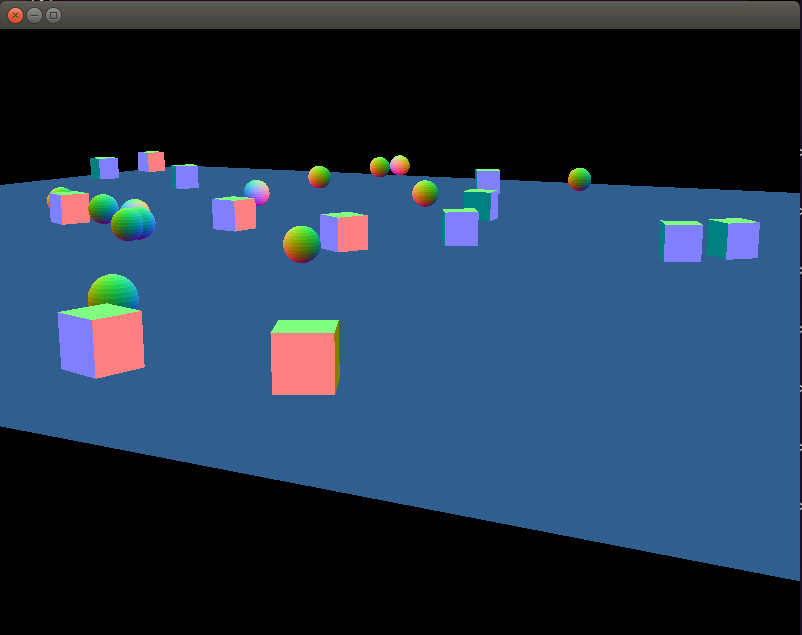
\includegraphics[width=0.5\textwidth]{test1}
\caption[Programa de prueba 1]{Juego que contiene esferas y cubos que aparecen random y se eliminan al chocar.}
\label{fig:test1}
\end{figure}

\begin{figure}[!htbp!]
\centering
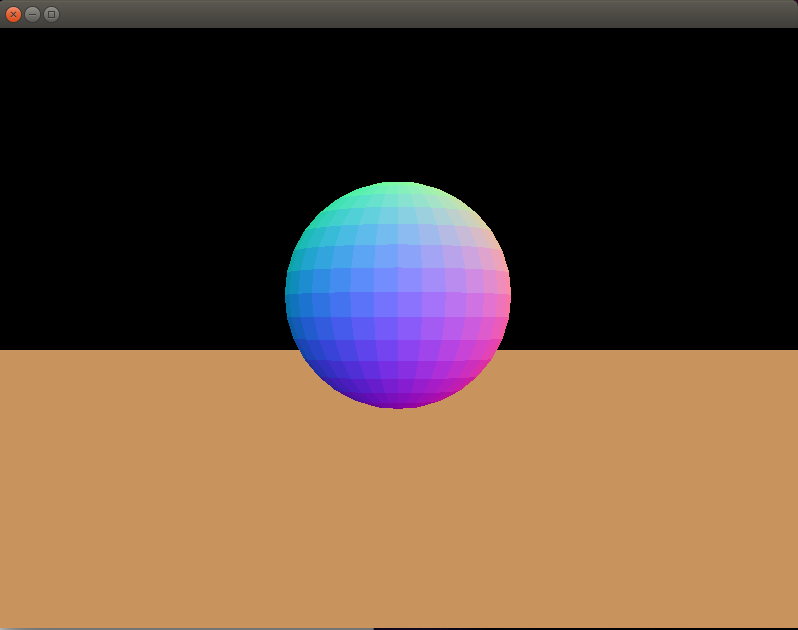
\includegraphics[width=0.5\textwidth]{test2}
\caption[Programa de prueba 2]{Juego de una pelota rebotando contra un piso.}
\label{fig:test2}
\end{figure}

\begin{figure}[!htbp!]
\centering
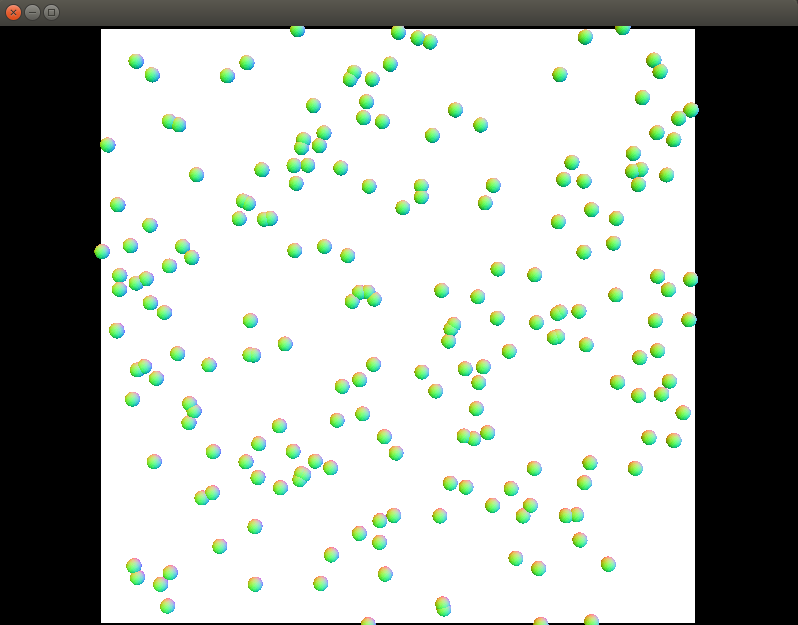
\includegraphics[width=0.5\textwidth]{test3}
\caption[Programa de prueba 3]{Juego en el que 200 esferas chocan y rebotan entre sí.}
\label{fig:test3}
\end{figure}

\begin{figure}[!htbp!]
\centering
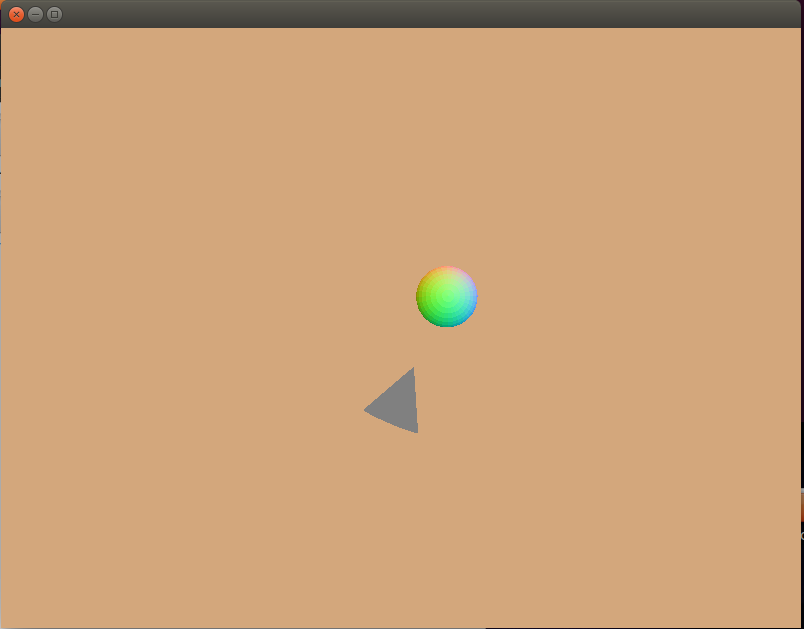
\includegraphics[width=0.5\textwidth]{gameia}
\caption[Programa de prueba 4]{Juego en el que un cono persigue a una esfera controlada por un jugador.}
\label{fig:gameia}
\end{figure}

\begin{figure}[!htbp!]
\centering
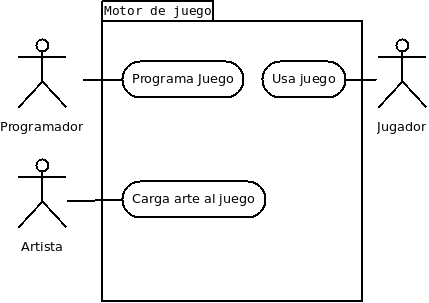
\includegraphics[width=0.8\textwidth]{MCU}
\caption[Diagrama de casos de uso]{}
\label{fig:MCU}
\end{figure}

%!TEX root = ../thesis.tex

\chapter{Código}

\lstinputlisting[label={EasyGL},caption={EasyGL.hs},language=Haskell]{./code/src/EasyGL.hs}
\lstinputlisting[label={EasyGLUT},caption={EasyGLUT.hs},language=Haskell]{./code/src/EasyGLUT.hs}
\lstinputlisting[label={EasyGL.Camera},caption={Camera.hs},language=Haskell]{./code/src/EasyGL/Camera.hs}
\lstinputlisting[label={EasyGL.EasyMem},caption={EasyMem.hs},language=Haskell]{./code/src/EasyGL/EasyMem.hs}
\lstinputlisting[label={EasyGL.Entity},caption={Entity.hs},language=Haskell]{./code/src/EasyGL/Entity.hs}
\lstinputlisting[label={EasyGL.IndexedModel},caption={IndexedModel.hs},language=Haskell]{./code/src/EasyGL/IndexedModel.hs}
\lstinputlisting[label={EasyGL.Material},caption={Material.hs},language=Haskell]{./code/src/EasyGL/Material.hs}
\lstinputlisting[label={EasyGL.Obj},caption={Obj.hs},language=Haskell]{./code/src/EasyGL/Obj.hs}
\lstinputlisting[label={EasyGL.Obj.Grammar},caption={Grammar.y},language=Haskell]{./code/src/EasyGL/Obj/Grammar.y}
\lstinputlisting[label={EasyGL.Obj.Obj2IM},caption={Obj2IM.hs},language=Haskell]{./code/src/EasyGL/Obj/Obj2IM.hs}
\lstinputlisting[label={EasyGL.ObjData},caption={ObjData.hs},language=Haskell]{./code/src/EasyGL/Obj/ObjData.hs}
\lstinputlisting[label={EasyGL.Obj.Tokens},caption={Tokens.x},language=Haskell]{./code/src/EasyGL/Obj/Tokens.x}
\lstinputlisting[label={EasyGL.Shader},caption={Shader.hs},language=Haskell]{./code/src/EasyGL/Shader.hs}
\lstinputlisting[label={EasyGL.Texture},caption={Texture.hs},language=Haskell]{./code/src/EasyGL/Texture.hs}
\lstinputlisting[label={EasyGL.Util},caption={Util.hs},language=Haskell]{./code/src/EasyGL/Util.hs}

\lstinputlisting[label={Val.Strict},caption={EasyGL.hs},language=Haskell]{./code/src/Val/Strict.hs}
\lstinputlisting[label={Val.Strict.Data},caption={EasyGL.hs},language=Haskell]{./code/src/Val/Strict/Data.hs}
\lstinputlisting[label={Val.Strict.Events},caption={EasyGL.hs},language=Haskell]{./code/src/Val/Strict/Events.hs}
\lstinputlisting[label={Val.Strict.IL},caption={EasyGL.hs},language=Haskell]{./code/src/Val/Strict/IL.hs}
\lstinputlisting[label={Val.Strict.Scene},caption={EasyGL.hs},language=Haskell]{./code/src/Val/Strict/Scene.hs}
\lstinputlisting[label={Val.Strict.UI},caption={EasyGL.hs},language=Haskell]{./code/src/Val/Strict/UI.hs}
\lstinputlisting[label={Val.Strict.Util},caption={EasyGL.hs},language=Haskell]{./code/src/Val/Strict/Util.hs}
\lstinputlisting[label={Val.Strict.Scene.Resources},caption={EasyGL.hs},language=Haskell]{./code/src/Val/Strict/Scene/Resources.hs}

\begin{lstlisting}[label={Ejemplo1},caption={Ejemplo - Mostrando armadillo},language=Haskell]
import EasyGL
import EasyGLUT
import System.Exit
import System.IO (stderr)
import Control.Monad.IO.Class (MonadIO,liftIO)
import qualified Graphics.Rendering.OpenGL as GL

armadillo :: Shader -> IO (Material,Entity)
armadillo myShader = do
  m <- makeMaterial myShader []
  case m of
    Left s -> putStrLn s >> exitFailure
    Right mat -> do
      e <- readObj2Ent "./armadillo.obj"
      return (mat,e)

main = do
	-- se inicializa el contexto de OpenGL y GLUT.
  initOpenGLEnvironment 800 600 "test"
	-- se carga los shaders.
  myShader <-
		loadShadersFromFile
			["./vertex.shader","./frag.shader"]
			[VertexShader,FragmentShader]
			(Just stderr)
	-- se carga el mayado.
  assets <- armadillo myShader
  initGL $ myfun assets

-- funcion para el ciclo principal de la aplicacion.
myfun :: (Material,Entity) -> GLUT ()
myfun (mat,ent) = do
	liftIO $ GL.preservingMatrix $ do
		useCamera cam
		drawWithMat mat ent $
			set "color" $ GL.Color4 1 1 0 (1 :: GL.GLfloat)
	where
		(Right cam) =
			createCamera3D 0.0 0.0 10.0 0 0 0 30 (800/600) 0.3 200
\end{lstlisting}

\begin{lstlisting}[label={Ejemplo2},caption={Ejemplo - Objetos que chocan},language=Haskell]
{-# LANGUAGE Arrows #-}

import Val.Strict hiding (yaw)
import EasyGL
import EasyGLUT
import Data.Either
import System.IO (stderr)
import FRP.Yampa hiding (RandomGen,randomR)
import Data.List (find)
import System.Random
import System.Environment
import qualified Graphics.Rendering.OpenGL as GL
import qualified Data.Map as Map
import qualified System.Random.TF as TF

-- Se cargan los recursos a utilizar en el ejemplo
load :: IO ResourceMap
load = do
  myShader <- loadShadersFromFile
    ["./assets/3Dshaders/vertex.shader",
    "./assets/3Dshaders/ColorShader.shader"]
    [VertexShader,FragmentShader]
    (Just stderr)
  (Right mat) <- makeMaterial myShader []
  let plane = ("plane","./assets/plane.obj",mat)

  myShader <- loadShadersFromFile
    ["./assets/3Dshaders/vertex.shader",
    "./assets/3Dshaders/NormalShader.shader"]
    [VertexShader,FragmentShader]
    (Just stderr)
  (Right mat) <- makeMaterial myShader []
  let sphere = ("sphere","./assets/cube.obj",mat)

  loadResouces [plane,sphere]

-- Informacion de los objetos.
data GameState = Null
  | Sphere {
    x :: Double,
    y :: Double,
    z :: Double,
    size :: Double
  }

collition :: GameState -> GameState -> Bool
collition Sphere{x=x1,z=y1} Sphere{x=x2,z=y2} =
  ( (x1-x2)^2 + (y1-y2)^2 ) < 4
collition _ _ = False

data EventTypes = Collition GameState
  | NoCollition

instance MergeableEvent EventTypes where
  union NoCollition NoCollition = NoCollition
  union a NoCollition = a
  union NoCollition a = a
  union a b = a

-- Funcion que detecta colisiones.
collitionGen :: IL GameState -> IL (Event EventTypes)
collitionGen inObjs = mapILWithKey aux inObjs
  where
    assocs = assocsIL inObjs
    aux key obj = case valid of
      (x:_) -> Event $ Collition . snd $ x
      [] -> noEvent
      where
        valid = filter
          (\(key2,obj2) -> key /= key2 && collition obj obj2 )
          assocs

cam :: SF (GameInput,IL GameState) Camera3D
cam = proc _ -> do
    returnA -< c
    where
    (Right c) = createCamera3D 0 150 0 0 (-90) 0 30 (800/600) 0.3 200

plane :: Object GameState EventTypes
plane = proc _ -> do
  let ret = newObjOutput Null
      trans = Transform
        (GL.Vector3 0 (-1) 0)
        (Quaternion 0 (GL.Vector3 0 1 0))
        2 1 2
      uni = do
        set "color" $ GL.Color4 1 1 1 (1 :: GL.GLfloat)
  returnA -< ret{ooRenderer=Just("plane",trans,uni)}

moveSF :: GL.GLdouble
  -> GL.GLdouble
  -> (GL.GLdouble,GL.GLdouble)
  -> SF () (GL.GLdouble,GL.GLdouble)
moveSF limMax limMin d@(dir,_) =
  if (dir > 0) then aux2 (> limMax) (< limMin) d else aux2 (< limMin) (> limMax) d
  where
    aux2 f1 f2 (dir,initx) = switch (aux f1 dir initx) (aux2 f2 f1)
    aux f dir initx = proc _ -> do
      xnew <- (+initx) ^<< integral -< dir
      e <- edge -< f xnew
      returnA -< ((xnew,dir),tag e (-dir,xnew))

moveXZSF :: GL.GLdouble -> GL.GLdouble -> (GL.GLdouble,GL.GLdouble) ->
  GL.GLdouble -> GL.GLdouble -> (GL.GLdouble,GL.GLdouble) ->
  SF a (GL.GLdouble,GL.GLdouble,GL.GLdouble,GL.GLdouble)
moveXZSF limMaxX limMinX initX limMaxZ limMinZ initZ = proc _ -> do
  (x,dirx) <- moveSF limMaxX limMinX initX -< ()
  (z,dirz) <- moveSF limMaxZ limMinZ initZ -< ()
  returnA -< (x,z,dirx,dirz)

type Info = (GL.GLdouble,GL.GLdouble,GL.GLdouble,GL.GLdouble)

getCollition :: SF (ObjInput GameState EventTypes,Info) (Event Info)
getCollition = proc (oi,salida) -> do
  let myEvent = event noEvent toEvent $ inputEvent oi
  returnA -< tag myEvent salida
  where
    toEvent NoCollition = noEvent
    toEvent a = Event a

sphere :: GL.GLdouble -> GL.GLdouble
  -> GL.GLdouble -> GL.GLdouble
  -> Object GameState EventTypes
sphere initx initz velx velz = proc gi -> do
  rec
    rot <- impulseIntegral -< (180,tag e (-360))
    e <- iPre noEvent <<< edge -< rot > 360
    (x,z,dirx,dirz) <- moveArr (initx,initz,velx,velz) -< gi

  let ret = newObjOutput $ Sphere (realToFrac x) 0 (realToFrac z) 1
      trans = Transform
        (GL.Vector3 x 0 z)
        (Quaternion rot (GL.Vector3 0 1 0))
        1 1 1
  returnA -< ret{ooRenderer=Just("sphere",trans,return ())}
  where
    moveArr (x,z,velx,velz) = dkSwitch
      (moveXZSF 40 (-40) (velx,x) 40 (-40) (velz,z))
      (getCollition >>> notYet)
      (\sf (x,z,velx,velz) -> moveArr (x,z,-velx,-velz) )

randomSphere :: RandomGen g => g -> (Object GameState EventTypes, g)
randomSphere g = (sphere initx initz velx velz,g4)
  where
    (initx,g1) = randomR (-39,39) g
    (initz,g2) = randomR (-39,39) g1
    (velx,g3) = randomR (-4,4) g2
    (velz,g4) = randomR (-4,4) g3

randomSphereList :: RandomGen g => g -> [Object GameState EventTypes]
randomSphereList g = obj:(randomSphereList g1)
	where
		(obj,g1) = randomSphere g

main :: IO ()
main = do
  num <- fmap (read . head) getArgs
  gen <- TF.mkSeedTime >>= return . TF.seedTFGen
  let il = [plane] ++ (take num $ randomSphereList gen)
  initScenePar cam load [collitionGen] il
\end{lstlisting}


%%!TEX root = ../thesis.tex
% ******************************* Thesis Appendix A ****************************
\chapter{How to install \LaTeX} 

\section*{Windows OS}

\subsection*{TeXLive package - full version}
\begin{enumerate}
\item	Download the TeXLive ISO (2.2GB) from\\
\href{https://www.tug.org/texlive/}{https://www.tug.org/texlive/}
\item	Download WinCDEmu (if you don't have a virtual drive) from \\
\href{http://wincdemu.sysprogs.org/download/}
{http://wincdemu.sysprogs.org/download/}
\item	To install Windows CD Emulator follow the instructions at\\
\href{http://wincdemu.sysprogs.org/tutorials/install/}
{http://wincdemu.sysprogs.org/tutorials/install/}
\item	Right click the iso and mount it using the WinCDEmu as shown in \\
\href{http://wincdemu.sysprogs.org/tutorials/mount/}{
http://wincdemu.sysprogs.org/tutorials/mount/}
\item	Open your virtual drive and run setup.pl
\end{enumerate}

or

\subsection*{Basic MikTeX - \TeX~ distribution}
\begin{enumerate}
\item	Download Basic-MiK\TeX (32bit or 64bit) from\\
\href{http://miktex.org/download}{http://miktex.org/download}
\item	Run the installer 
\item	To add a new package go to Start >> All Programs >> MikTex >> Maintenance (Admin) and choose Package Manager
\item	Select or search for packages to install
\end{enumerate}

\subsection*{TexStudio - \TeX~ editor}
\begin{enumerate}
\item	Download TexStudio from\\
\href{http://texstudio.sourceforge.net/\#downloads}
{http://texstudio.sourceforge.net/\#downloads} 
\item	Run the installer
\end{enumerate}

\section*{Mac OS X}
\subsection*{MacTeX - \TeX~ distribution}
\begin{enumerate}
\item	Download the file from\\
\href{https://www.tug.org/mactex/}{https://www.tug.org/mactex/}
\item	Extract and double click to run the installer. It does the entire configuration, sit back and relax.
\end{enumerate}

\subsection*{TexStudio - \TeX~ editor}
\begin{enumerate}
\item	Download TexStudio from\\
\href{http://texstudio.sourceforge.net/\#downloads}
{http://texstudio.sourceforge.net/\#downloads} 
\item	Extract and Start
\end{enumerate}


\section*{Unix/Linux}
\subsection*{TeXLive - \TeX~ distribution}
\subsubsection*{Getting the distribution:}
\begin{enumerate}
\item	TexLive can be downloaded from\\
\href{http://www.tug.org/texlive/acquire-netinstall.html}
{http://www.tug.org/texlive/acquire-netinstall.html}.
\item	TexLive is provided by most operating system you can use (rpm,apt-get or yum) to get TexLive distributions
\end{enumerate}

\subsubsection*{Installation}
\begin{enumerate}
\item	Mount the ISO file in the mnt directory
\begin{verbatim}
mount -t iso9660 -o ro,loop,noauto /your/texlive####.iso /mnt
\end{verbatim}

\item	Install wget on your OS (use rpm, apt-get or yum install)
\item	Run the installer script install-tl.
\begin{verbatim}
	cd /your/download/directory
	./install-tl
\end{verbatim}
\item	Enter command `i' for installation

\item	Post-Installation configuration:\\
\href{http://www.tug.org/texlive/doc/texlive-en/texlive-en.html\#x1-320003.4.1}
{http://www.tug.org/texlive/doc/texlive-en/texlive-en.html\#x1-320003.4.1} 
\item	Set the path for the directory of TexLive binaries in your .bashrc file
\end{enumerate}

\subsubsection*{For 32bit OS}
For Bourne-compatible shells such as bash, and using Intel x86 GNU/Linux and a default directory setup as an example, the file to edit might be \begin{verbatim}
edit $~/.bashrc file and add following lines
PATH=/usr/local/texlive/2011/bin/i386-linux:$PATH; 
export PATH 
MANPATH=/usr/local/texlive/2011/texmf/doc/man:$MANPATH;
export MANPATH 
INFOPATH=/usr/local/texlive/2011/texmf/doc/info:$INFOPATH;
export INFOPATH
\end{verbatim}
\subsubsection*{For 64bit OS}
\begin{verbatim}
edit $~/.bashrc file and add following lines
PATH=/usr/local/texlive/2011/bin/x86_64-linux:$PATH;
export PATH 
MANPATH=/usr/local/texlive/2011/texmf/doc/man:$MANPATH;
export MANPATH 
INFOPATH=/usr/local/texlive/2011/texmf/doc/info:$INFOPATH;
export INFOPATH

\end{verbatim}



%\subsection{Installing directly using Linux packages} 
\subsubsection*{Fedora/RedHat/CentOS:}
\begin{verbatim} 
sudo yum install texlive 
sudo yum install psutils 
\end{verbatim}


\subsubsection*{SUSE:}
\begin{verbatim}
sudo zypper install texlive
\end{verbatim}


\subsubsection*{Debian/Ubuntu:}
\begin{verbatim} 
sudo apt-get install texlive texlive-latex-extra 
sudo apt-get install psutils
\end{verbatim}

%%!TEX root = ../thesis.tex
% ******************************* Thesis Appendix B ********************************

\chapter{Installing the CUED class file}

\LaTeX.cls files can be accessed system-wide when they are placed in the
<texmf>/tex/latex directory, where <texmf> is the root directory of the user’s \TeX installation. On systems that have a local texmf tree (<texmflocal>), which
may be named ``texmf-local'' or ``localtexmf'', it may be advisable to install packages in <texmflocal>, rather than <texmf> as the contents of the former, unlike that of the latter, are preserved after the \LaTeX system is reinstalled and/or upgraded.

It is recommended that the user create a subdirectory <texmf>/tex/latex/CUED for all CUED related \LaTeX class and package files. On some \LaTeX systems, the directory look-up tables will need to be refreshed after making additions or deletions to the system files. For \TeX Live systems this is accomplished via executing ``texhash'' as root. MIK\TeX users can run ``initexmf -u'' to accomplish the same thing.

Users not willing or able to install the files system-wide can install them in their personal directories, but will then have to provide the path (full or relative) in addition to the filename when referring to them in \LaTeX.



\end{appendices}

% *************************************** Index ********************************
\printthesisindex % If index is present

\end{document}
